\documentclass[aspectratio=169,11pt]{beamer}  % 11pt: Inter (EAFIT font) is wider than Latin Modern
\usepackage{eafitml}
\usepackage{colortbl}
% scalable big operators (lmex is size-fixed by default)
\DeclareFontFamily{OMX}{lmex}{}
\DeclareFontShape{OMX}{lmex}{m}{n}{<->lmex10}{}
\setbeamerfont{title}{series=\bfseries,size=\Large}
\lstset{columns=flexible}

% ------------------------------------------------------------ local macros
\makeatletter
% frame title + gray subtitle (as in the original slides)
\setbeamertemplate{frametitle}{\vskip0.25em\usebeamerfont{frametitle}\usebeamercolor[fg]{frametitle}\insertframetitle\par
  \ifx\insertframesubtitle\@empty\else\vskip0.1em{\normalfont\footnotesize\color{mlgray}\insertframesubtitle\par}\fi}
\makeatother
% table of contents (same style as sessions 1-2)
\setbeamertemplate{section in toc}{\leavevmode{\color{mlgold}\inserttocsectionnumber.}~\inserttocsection\par}
\setbeamertemplate{subsection in toc}{\leavevmode\leftskip=2.2em\small\mdseries\inserttocsubsection\par}
\setbeamerfont{section in toc}{series=\bfseries,size=\normalsize}

% figure on white page, placed at bbox (38,20)-(413,230) pt
\newcommand{\figframe}[1]{%
  {\setbeamertemplate{background}{\vbox to\paperheight{\vskip20bp\hbox{\hskip38bp\includegraphics[width=375bp,height=210bp]{#1}}\vss}}%
   \begin{frame}[plain]\end{frame}}}
% gold header + light teal body ("Uso práctico", "Ejemplo esperado", ...)
\newtcolorbox{goldbox}[1][]{enhanced,sharp corners,boxrule=0pt,frame hidden,
  colback=mltealbg,colbacktitle=mlgold,coltitle=white,
  fonttitle=\bfseries\small,left=4pt,right=4pt,top=2pt,bottom=2pt,
  toptitle=1pt,bottomtitle=1pt,before skip=4pt,after skip=4pt,title={#1}}
\setbeamersize{text margin left=18.6pt,text margin right=18.6pt}
\newcolumntype{P}[1]{>{\raggedright\arraybackslash}p{#1}}
% table conventions
\arrayrulecolor{mltitle}
\newcommand{\hrow}{\rowcolor{mlcream}}
\newcommand{\Lg}{\fontsize{16}{20}\selectfont}
\newcommand{\bigstate}[1]{\begin{center}\Lg #1\end{center}}
\newcommand{\bigq}[1]{\begin{center}\Lg\bfseries #1\end{center}}

% placeholder for data the instructor must confirm (links)
\newcommand{\pend}[1]{\textcolor{mlred}{\textbf{[#1]}}}
\newcommand{\colhead}[1]{\textbf{#1}\par\vspace{2pt}}

\title[Series de tiempo, forecasting tabular y walk-forward validation]{Series de tiempo, forecasting tabular y walk-forward validation}
\subtitle{Aprendizaje Automático · Sesión 3}
\author[Aprendizaje Automático]{Andrés Vásquez Restrepo\\[2pt]{\normalfont\small\texttt{avasquezr3@eafit.edu.co}}}
\institute{SI7009 - 1 (5553)\\Universidad EAFIT}
\date{2026-2 -- Medellín}
\titlegraphic{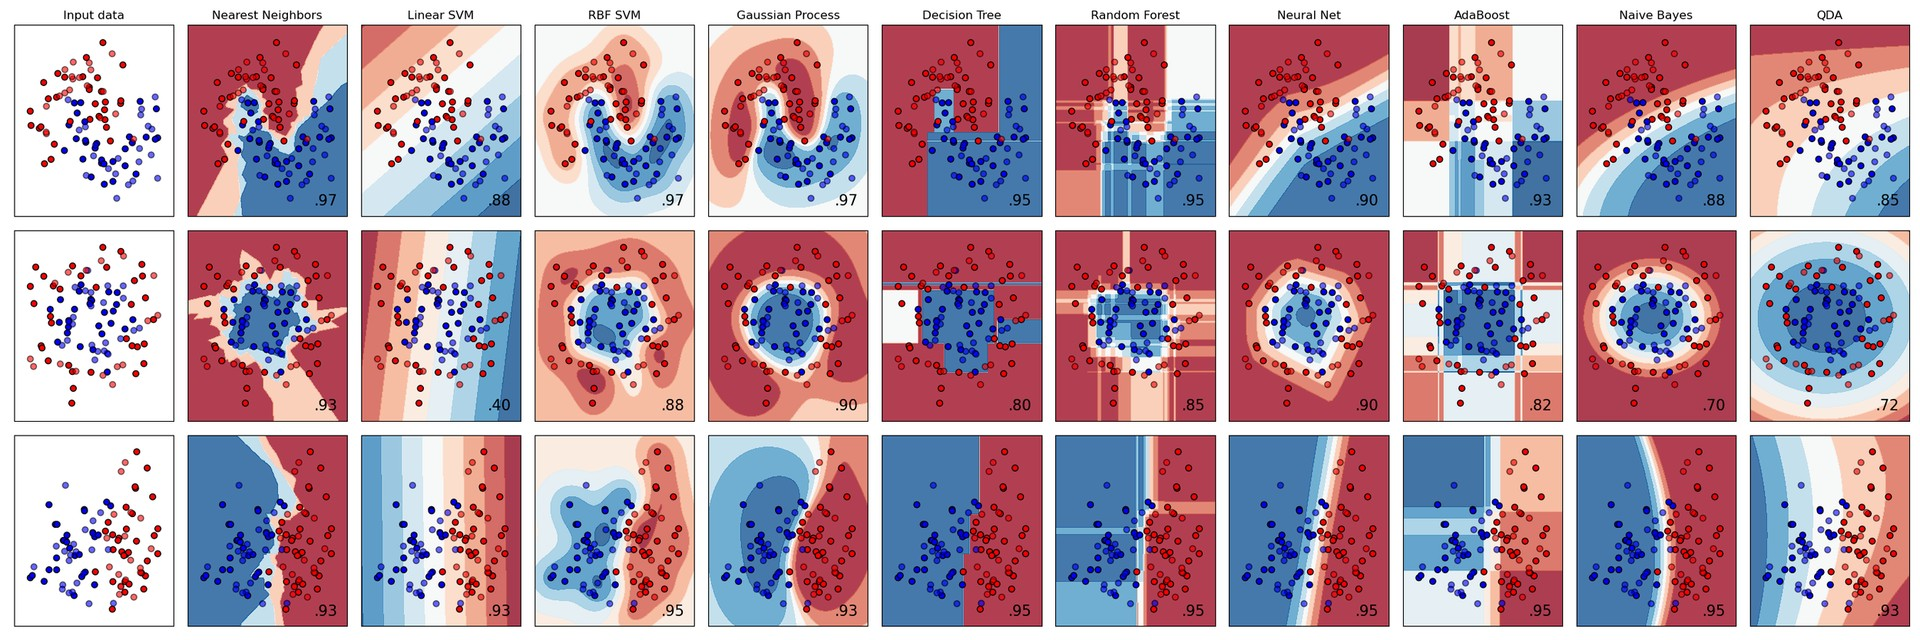
\includegraphics[width=5cm]{figures/img_p001_01.jpg}}

\begin{document}

% ============================================================ A. apertura (1, 2, A1)
\titleframe
\setcounter{framenumber}{1}

\begin{frame}[t]{Contenido}
\vspace*{-0.3em}
{\setlength{\parskip}{0pt}\tableofcontents}
\end{frame}

\begin{frame}{Dónde quedamos}
\framesubtitle{El tiempo ya apareció en el curso: hoy se vuelve el centro}
\begin{columns}[T]
\column{0.5\textwidth}
\colhead{Sesiones 1 y 2}
\begin{itemize}\small
\item S1: \texttt{TimeSeriesSplit} como CV temporal ``si las features tienen cronología'';
\item S2: el fold de Optuna depende de los datos (estratificado o temporal);
\item baseline serio, leakage dentro de la validación.
\end{itemize}
\column{0.44\textwidth}
\begin{keybox}[Hoy]
\small Predecir el futuro sin mirarlo: \textbf{una serie} (tráfico Metro) para el método y \textbf{muchas series} (consumo eléctrico) para el modelo global.
\end{keybox}
\end{columns}
\vspace{4pt}
{\footnotesize\color{mlgray} Ruta: estructura $\rightarrow$ formulación $\rightarrow$ windowing $\rightarrow$ features $\rightarrow$ modelo global $\rightarrow$ baselines $\rightarrow$ validación $\rightarrow$ métricas $\rightarrow$ modelos y hands-on.\par}
\end{frame}

% ============================================================ 1. el tiempo cambia el experimento (3, 4+6+7, 9)
\section{El tiempo cambia el experimento}
\sectionframe{\LARGE El tiempo cambia el experimento}

\begin{frame}{La pregunta central de esta sesión}
\framesubtitle{El problema no es tener fechas; es predecir sin mirar el futuro}
\begin{center}\large En datos temporales, un score alto no demuestra valor si el experimento permitió mirar el futuro.\end{center}
\[ y_1,\ y_2,\ \ldots,\ y_t,\ \ldots,\ y_T \qquad\qquad \hat y_{t+h} = f(X_t) \text{ con } X_t \text{ disponible solo hasta } t \]
\begin{itemize}\small
\item El \textbf{orden} define qué información era observable: las filas ya no son intercambiables.
\item El \textbf{horizonte} define qué tan lejos queremos predecir.
\item La \textbf{validación} define si el score representa operación real.
\end{itemize}
\begin{rulebox}[Lo aprendido antes se vuelve más exigente]
\small ¿El modelo habría tenido esta información en el momento real en que debía predecir? Si no, el resultado está inflado aunque el código sea correcto.
\end{rulebox}
\end{frame}

\begin{frame}{Chequeo inicial: ¿qué podía saber el modelo?}
\framesubtitle{Antes de entrenar, audite la disponibilidad de información}
\begin{taskbox}[{\large Discusión breve}]
Queremos predecir el volumen de tráfico una hora adelante. Para una predicción hecha a las 8:00 AM, decida qué información es válida.
\end{taskbox}
\begin{enumerate}
\item Volumen observado a las 7:00 AM.
\item Promedio de tráfico entre 8:00 AM y 10:00 AM.
\item Hora del día y día de la semana.
\item Clima reportado después del periodo objetivo.
\item Volumen de la misma hora del día anterior.
\end{enumerate}
Una columna histórica solo es válida si su versión operacional existía antes de la predicción.
\end{frame}

% ============================================================ 2. leer la estructura temporal (10, 11+13+14, 15, 16, 19)
\section{Leer la estructura temporal}
\sectionframe{\LARGE Antes de modelar: leer la estructura\\temporal}

\begin{frame}{Una serie de tiempo no es solo una fecha}
\framesubtitle{Es una señal ordenada con memoria, ciclos y posible cambio}
\begin{columns}[c]
\column{0.38\textwidth}
{\large\[ y_t = T_t + S_t + R_t \]}
\begin{itemize}\small
\item $T_t$: \textbf{tendencia}, cambio lento del nivel;
\item $S_t$: \textbf{estacionalidad}, patrón repetido;
\item $R_t$: \textbf{residuo}, lo que queda sin explicar.
\end{itemize}
\vspace{2pt}
{\footnotesize Si se pierde el \textbf{orden}, se pierde la estructura que hace posible el forecasting.\par}
\column{0.6\textwidth}
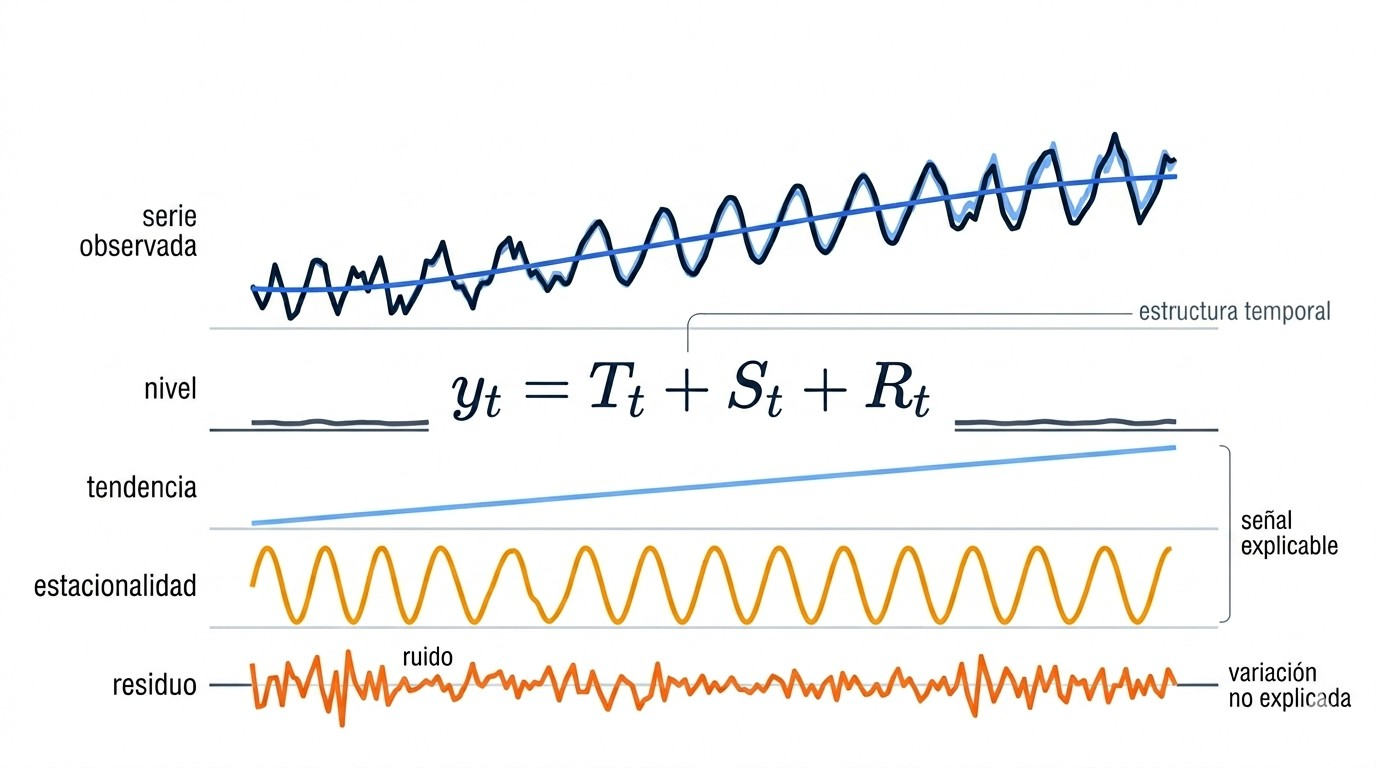
\includegraphics[width=\linewidth]{figures/img_p012_04.jpg}
\end{columns}
\begin{rulebox}[Cuidado]
\small La descomposición ayuda a leer tendencia y ciclos; la evidencia predictiva sigue dependiendo de validación hacia adelante.
\end{rulebox}
\end{frame}

\begin{frame}{Frecuencia y granularidad}
\framesubtitle{La pregunta cambia si los datos son horarios, diarios o mensuales}
\begin{columns}[c]
\column{0.36\textwidth}
\centering\footnotesize
\begin{tabular}{@{}l P{0.6\linewidth}@{}}
\toprule
\hrow \textbf{Frecuencia} & Riesgo frecuente\\
\midrule
\textbf{Horaria} & confundir ciclos diarios con ruido\\
\textbf{Diaria} & ignorar fines de semana y eventos\\
\textbf{Semanal} & tener pocos puntos por ciclo\\
\textbf{Mensual} & sobreinterpretar series cortas\\
\bottomrule
\end{tabular}
\column{0.62\textwidth}
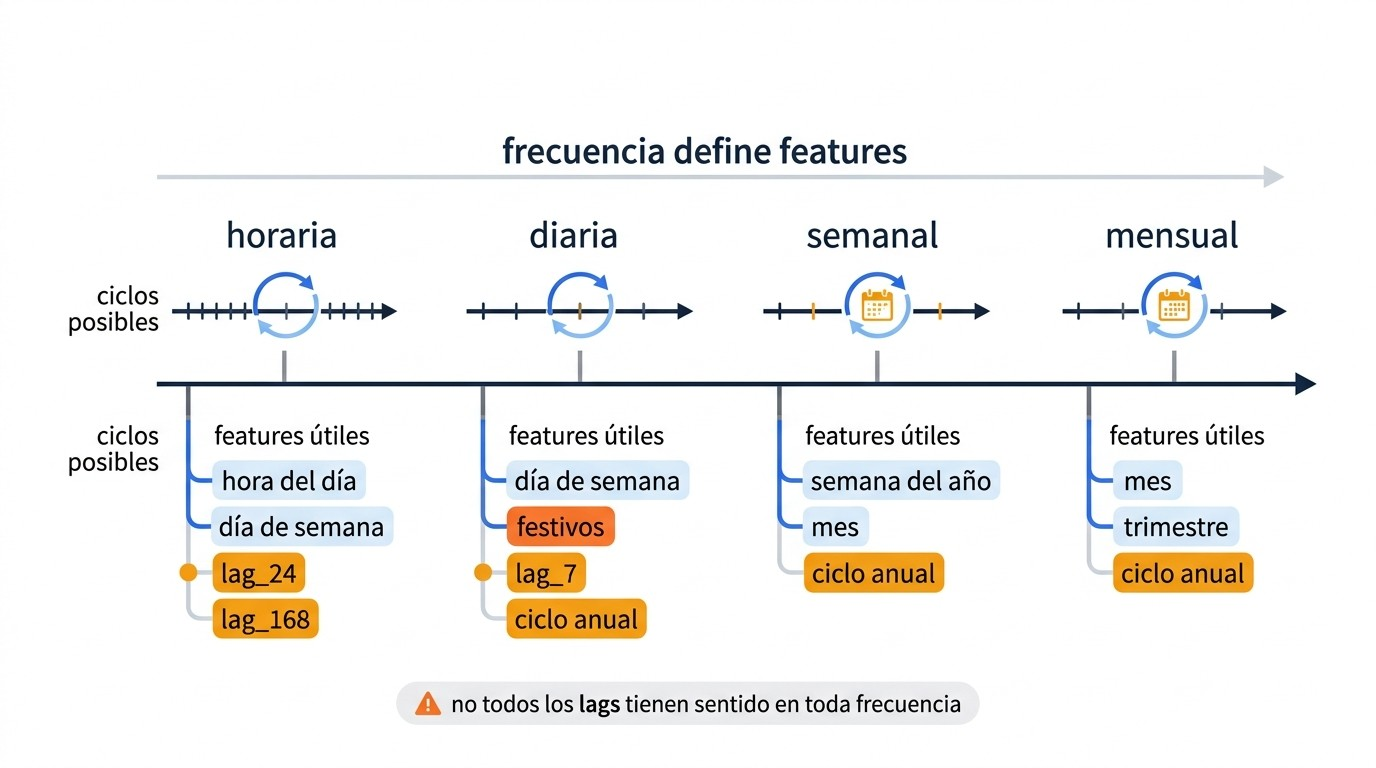
\includegraphics[width=\linewidth]{figures/img_p014_05.jpg}
\end{columns}
\vspace{0.6em}
\textbf{Regla:} La frecuencia define qué \emph{lags}, ventanas, estacionalidades y métricas tienen sentido.
\end{frame}

\begin{frame}{Autocorrelación: memoria estadística}
\framesubtitle{El pasado puede seguir hablando en el presente}
\begin{columns}[c]
\column{0.38\textwidth}
{\large\[ \rho_k = \operatorname{corr}(y_t,\ y_{t-k}) \]}
\begin{itemize}\small
\item \textbf{ACF}: $\rho_1$ alto sugiere persistencia; $\rho_{24}$ alto en datos horarios, ciclo diario;
\item \textbf{PACF}: correlación con $y_{t-k}$ descontando los lags intermedios; sugiere qué lags aportan algo propio;
\item orienta lags y baselines; no prueba causalidad.
\end{itemize}
\column{0.6\textwidth}
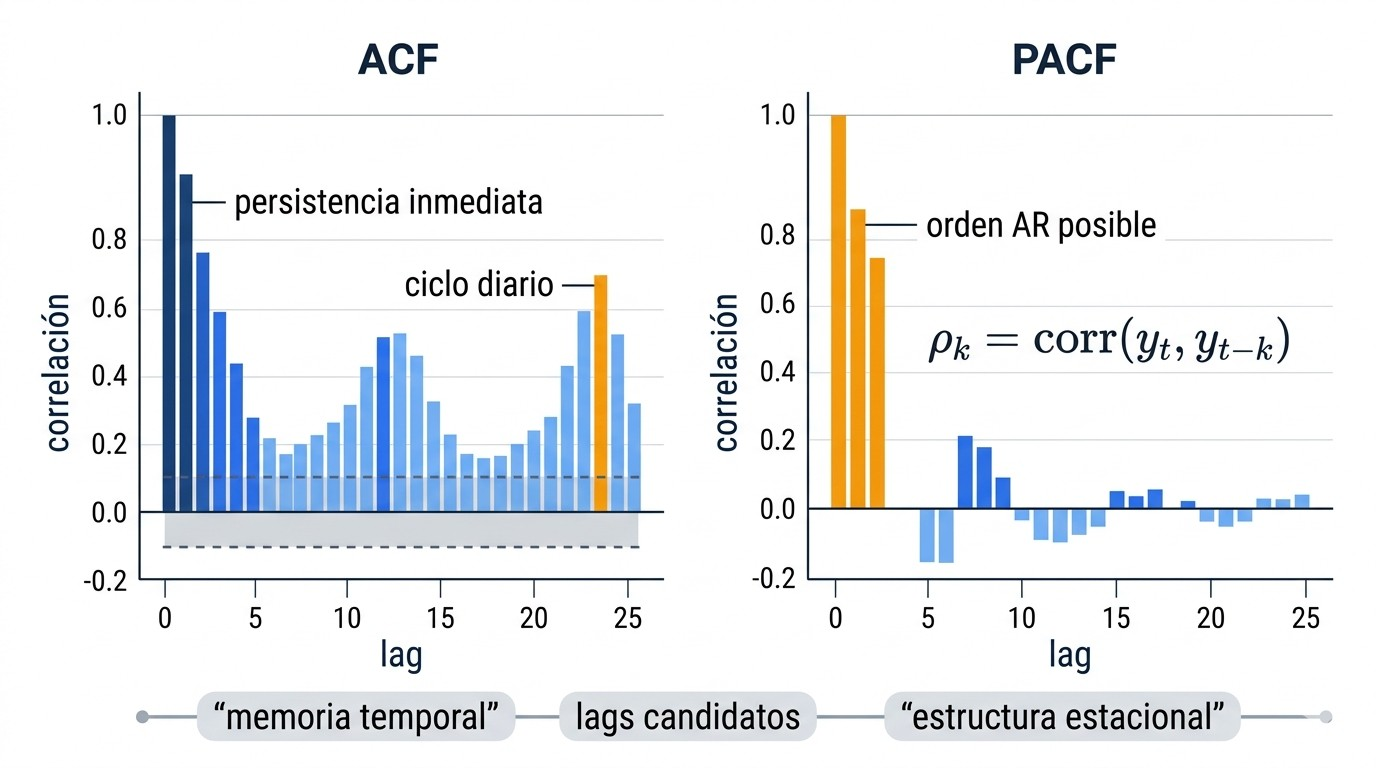
\includegraphics[width=\linewidth]{figures/img_p017_06.jpg}
\end{columns}
\begin{goldbox}[Uso práctico]
\small Si $\rho_{s}$ es alto (por ejemplo $s = 24$), el lag estacional $y_{t-s}$ y el seasonal naïve merecen probarse antes de entrenar modelos complejos.
\end{goldbox}
\end{frame}

\begin{frame}{Checklist de diagnóstico antes de modelar}
\framesubtitle{El modelo no debe ser la primera herramienta}
Antes de entrenar, responda
\begin{enumerate}
\item ¿Cuál es la frecuencia real de la serie?
\item ¿Hay huecos, duplicados o cambios de granularidad?
\item ¿Hay tendencia visible?
\item ¿Hay estacionalidad diaria, semanal o anual?
\item ¿La ACF sugiere persistencia o ciclos?
\item ¿El baseline seasonal naïve parece competitivo?
\item ¿El horizonte elegido coincide con la decisión operativa?
\end{enumerate}
\vspace{0.5em}
\begin{center}
Una serie de tiempo se entiende primero como fenómeno; solo después como matriz de entrenamiento.
\end{center}
\end{frame}

% ============================================================ 3. formulación (20, 21+22, 24+25, 26)
\section{Formulación: target y horizonte}
\sectionframe{\LARGE Target temporal, predicción y\\horizonte}

\begin{frame}{``Predecir tráfico'' no es una formulación completa}
\framesubtitle{El target pertenece al futuro; las features pertenecen al pasado disponible}
{\Large\[ \hat y_{t+h} = f(X_t) \]}
\begin{columns}[T]
\column{0.23\textwidth} \small $t$\\ momento en que el sistema debe tomar la predicción.
\column{0.23\textwidth} \small $h$\\ \textbf{horizonte}: distancia entre predicción y objetivo.
\column{0.23\textwidth} \small $X_t$\\ información conocida hasta $t$.
\column{0.23\textwidth} \small $y_{t+h}$\\ valor futuro que queremos estimar.
\end{columns}
\vspace{6pt}
\begin{rulebox}[Formulación incompleta]
\small ``Predecir demanda'' o ``predecir tráfico'' no alcanza: una formulación temporal fija qué se predice, desde cuándo, con qué información y a qué horizonte.
\end{rulebox}
\end{frame}

\begin{frame}{El horizonte cambia la formulación}
\framesubtitle{Un buen modelo a 1 hora no necesariamente sirve a 24 horas}
\centering\small
\begin{tabular}{@{}l P{0.39\textwidth} P{0.41\textwidth}@{}}
\toprule
\hrow \textbf{Horizonte} & Pregunta operativa & Lectura metodológica\\
\midrule
\textbf{1 hora} & ¿Qué pasará casi inmediatamente? & alta dependencia del estado reciente\\
\textbf{3 horas} & ¿Cómo evoluciona el corto plazo? & empieza a importar la tendencia local\\
\textbf{6 horas} & ¿Qué patrón domina medio día operativo? & pueden aparecer ciclos y cambios de régimen\\
\textbf{24 horas} & ¿Qué ocurrirá en el mismo punto del siguiente día? & la estacionalidad diaria puede importar más que el último valor\\
\bottomrule
\end{tabular}
\raggedright
\begin{taskbox}[Práctica]
\small Complete la formulación (target, momento, horizonte, información): ``predecir demanda de bicicletas'' y ``predecir ventas para inventario''.
\end{taskbox}
\end{frame}

\begin{frame}{El caso aplicado debe servir al método, no al revés}
\framesubtitle{Cada dataset cumple una función pedagógica distinta}
\centering\footnotesize
\begin{tabular}{@{}P{0.27\textwidth} P{0.36\textwidth} P{0.30\textwidth}@{}}
\toprule
\hrow \textbf{Dataset} & Por qué sirve & Uso en la sesión\\
\midrule
\textbf{Metro Interstate Traffic Volume} & una serie horaria con clima, festivos y estacionalidad diaria & método: horizonte, lags, baselines, walk-forward\\
\textbf{UCI Electricity Load Diagrams} & consumo horario de muchos clientes con escalas distintas & \textbf{modelo global} frente a modelos locales\\
\textbf{Serie sintética y dummy manual} & tendencia, ciclo y alineación controlados & random split frente a temporal; alineación lag--target\\
\textbf{Bike Sharing} & demanda horaria más liviana & respaldo pedagógico\\
\bottomrule
\end{tabular}

{\small El \emph{dataset} no se elige por fama; se elige porque permite demostrar decisiones temporales correctas.\par}
\end{frame}

% ============================================================ 4. windowing (27, 28+30, 31, 32, W1, W2)
\section{Windowing: de serie a tabla supervisada}
\sectionframe{\LARGE Windowing: de serie temporal\\a tabla supervisada}

\begin{frame}{Forecasting tabular: cada fila es una decisión en $t$}
\framesubtitle{El objetivo no es ``usar fechas''; es construir filas válidas de predicción}
{\large\[ \mathbf{z}_t = \bigl[y_{t-1},\ y_{t-24},\ \mathrm{rolling}_{24}(t),\ \mathrm{calendar}(t),\ \mathrm{exo}(t)\bigr] \longrightarrow y_{t+h} \]}
\begin{itemize}\small
\item un modelo tabular no entiende una serie por defecto: hay que convertir el pasado disponible en una fila;
\item $\mathbf{z}_t$ contiene solo señales disponibles al momento de predicción;
\item $y_{t-1}$: memoria inmediata · $y_{t-24}$: referencia estacional diaria;
\item $\mathrm{exo}(t)$ debe ser una versión externa disponible en $t$, no una observación futura.
\end{itemize}
\begin{rulebox}[Error común]
\small Crear columnas temporales sin revisar alineación produce un dataset elegante pero contaminado.
\end{rulebox}
\end{frame}

\begin{frame}{Ejemplo mínimo de alineación}
\framesubtitle{La primera intuición del notebook debe ser manual y visible}
\centering
\begin{tabular}{@{}c c c c P{0.36\textwidth}@{}}
\toprule
\hrow \textbf{Tiempo} & $y_t$ observado & $\mathrm{lag}_1$ & Target $y_{t+1}$ & Lectura\\
\midrule
\textbf{08:00} & 120 & -- & 135 & no hay historia suficiente para $\mathrm{lag}_1$\\
\textbf{09:00} & 135 & 120 & 150 & fila válida para predecir 10:00\\
\textbf{10:00} & 150 & 135 & 142 & fila válida para predecir 11:00\\
\textbf{11:00} & 142 & 150 & -- & no conocemos target futuro al construir evidencia histórica\\
\bottomrule
\end{tabular}

\vspace{1.5em}
Al desplazar \emph{features} y \emph{target}, algunas filas se pierden. Esa pérdida no es un error: es consecuencia de respetar el tiempo.
\end{frame}

\begin{frame}{Una tabla temporal puede estar mal aunque se vea completa}
\framesubtitle{La validez depende de cómo se construyó cada columna}
\begin{columns}[T]
\column{0.47\textwidth}
\textbf{Fila temporal válida}
\begin{itemize}
\item usa valores anteriores a $t$;
\item calcula agregados con ventana histórica;
\item incorpora calendario conocido;
\item usa variables exógenas disponibles antes de decidir.
\end{itemize}
\column{0.47\textwidth}
\textbf{Fila temporal contaminada}
\begin{itemize}
\item usa $y_{t+h}$ directa o indirectamente;
\item calcula promedios con datos futuros;
\item normaliza usando todo el dataset;
\item incluye variables publicadas después del evento.
\end{itemize}
\end{columns}
\begin{rulebox}[Regla metodológica]
La validez de una feature depende de su disponibilidad operacional, no de su presencia en el archivo.
\end{rulebox}
\end{frame}

\begin{frame}{Ventana deslizante: cómo se arma cada fila}
\framesubtitle{Una ventana de longitud $L$ mira hacia atrás; el objetivo está $h$ pasos adelante}
\centering
\begin{tikzpicture}[x=0.5cm,y=0.55cm]
  \foreach \i in {0,...,19} \draw[mlgraybg,fill=white] (\i,0) rectangle ++(0.9,0.9);
  \foreach \row/\s in {0/2,1/3,2/4}{
    \pgfmathsetmacro{\yy}{-1.2-1.1*\row}
    \foreach \i in {0,...,5} \fill[eafitsky] (\s+\i,\yy) rectangle ++(0.9,0.9);
    \fill[mlred] (\s+8,\yy) rectangle ++(0.9,0.9);
    \node[font=\tiny,anchor=east] at (\s-0.2,\yy+0.45) {fila \the\numexpr\row+1\relax};
  }
  \node[font=\scriptsize,anchor=west] at (20.2,0.45) {serie $y_t$};
  \fill[eafitsky] (0,-5.2) rectangle ++(0.9,0.6); \node[font=\scriptsize,anchor=west] at (1,-4.9) {ventana: $y_{t-L+1}, \ldots, y_t$ (features)};
  \fill[mlred] (10,-5.2) rectangle ++(0.9,0.6); \node[font=\scriptsize,anchor=west] at (11,-4.9) {objetivo $y_{t+h}$ (aquí $h = 3$)};
\end{tikzpicture}
\par\vspace{4pt}
\raggedright\small
\begin{itemize}
\item cada fila desplaza la ventana un paso: la serie se convierte en una tabla \textbf{sin mirar el futuro};
\item la longitud $L$ (lookback) es un \textbf{hiperparámetro}: se elige con walk-forward, no a ojo;
\item ventanas, lags y rolling son la misma idea: resumir el pasado disponible en $t$.
\end{itemize}
\end{frame}

\begin{frame}{Ejemplo: de la ventana a la tabla}
\framesubtitle{Serie horaria con ventana $L = 3$ y horizonte $h = 1$}
\centering\small
\begin{tabular}{@{}l *{8}{c}@{}}
\toprule
\hrow \textbf{hora} & 08:00 & 09:00 & 10:00 & 11:00 & 12:00 & 13:00 & 14:00 & 15:00\\
\midrule
$y_t$ & 120 & 135 & 150 & 142 & 160 & 171 & 158 & 149\\
\bottomrule
\end{tabular}
\par\vspace{2pt}
{\Large$\Downarrow$}
\par\vspace{2pt}
\begin{tabular}{@{}l >{\columncolor{eafitsky}}c >{\columncolor{eafitsky}}c >{\columncolor{eafitsky}}c >{\columncolor{mlredbg}}c@{}}
\toprule
\hrow \textbf{momento $t$} & $y_{t-2}$ & $y_{t-1}$ & $y_t$ & \textbf{target} $y_{t+1}$\\
\midrule
10:00 & 120 & 135 & 150 & 142\\
11:00 & 135 & 150 & 142 & 160\\
12:00 & 150 & 142 & 160 & 171\\
13:00 & 142 & 160 & 171 & 158\\
14:00 & 160 & 171 & 158 & 149\\
\bottomrule
\end{tabular}
\par\vspace{4pt}
\raggedright\footnotesize
\begin{itemize}
\item cada fila es la ventana anterior desplazada una hora: 8 valores producen 5 filas (se pierden $L - 1$ al inicio y $h$ al final);
\item las columnas azules son las \textbf{features} (solo pasado); la roja es el \textbf{target} (futuro);
\item con $h = 3$ el target de la fila 10:00 sería $y_{13:00} = 171$, y se pierden 3 filas al final.
\end{itemize}
\end{frame}

\begin{frame}{Estrategias multi-paso: predecir varios horizontes}
\framesubtitle{Cómo obtener $\hat y_{t+1}, \ldots, \hat y_{t+H}$ con un modelo tabular}
\centering\small
\begin{tabular}{@{}l P{0.32\textwidth} P{0.15\textwidth} P{0.26\textwidth}@{}}
\toprule
\hrow \textbf{Estrategia} & Cómo funciona & Modelos & Riesgo o ventaja\\
\midrule
\textbf{Recursiva} & un modelo a 1 paso; su predicción se usa como lag para el siguiente & 1 & acumula error en horizontes largos\\
\textbf{Directa} & un modelo distinto para cada horizonte $h$ & $H$ & sin acumulación; más modelos que entrenar\\
\textbf{Multi-output} & un modelo predice las $H$ salidas a la vez & 1 & comparte señal entre horizontes\\
\bottomrule
\end{tabular}
\raggedright
\begin{keybox}[En el notebook]
\small Se usa la estrategia \textbf{directa}: un target $y_{t+h}$ por cada $h \in \{1, 3, 6, 24\}$. Es la más fácil de auditar.
\end{keybox}
\end{frame}

% ============================================================ 5. features (33, 34+36, 37+42, 38+40, 41+F1)
\section{Features: lags, rolling y calendario}
\sectionframe{\LARGE Features temporales válidas}

\begin{frame}{Lags y rolling windows convierten memoria en evidencia}
\framesubtitle{Cada feature temporal debe representar pasado disponible}
\begin{columns}[c]
\column{0.4\textwidth}
\[ \mathrm{lag}_k(t) = y_{t-k} \]
\[ \mathrm{rolling\_mean}_w(t) = \frac{1}{w}\sum_{i=1}^{w} y_{t-i} \]
\begin{itemize}\small
\item \textbf{lags}: memoria puntual ($\mathrm{lag}_1$, $\mathrm{lag}_{24}$);
\item \textbf{rolling}: nivel y variabilidad recientes (media y desviación de 24 h);
\item válidos solo si terminan antes de $t$: \texttt{y.shift(1).rolling(w)}.
\end{itemize}
\column{0.58\textwidth}
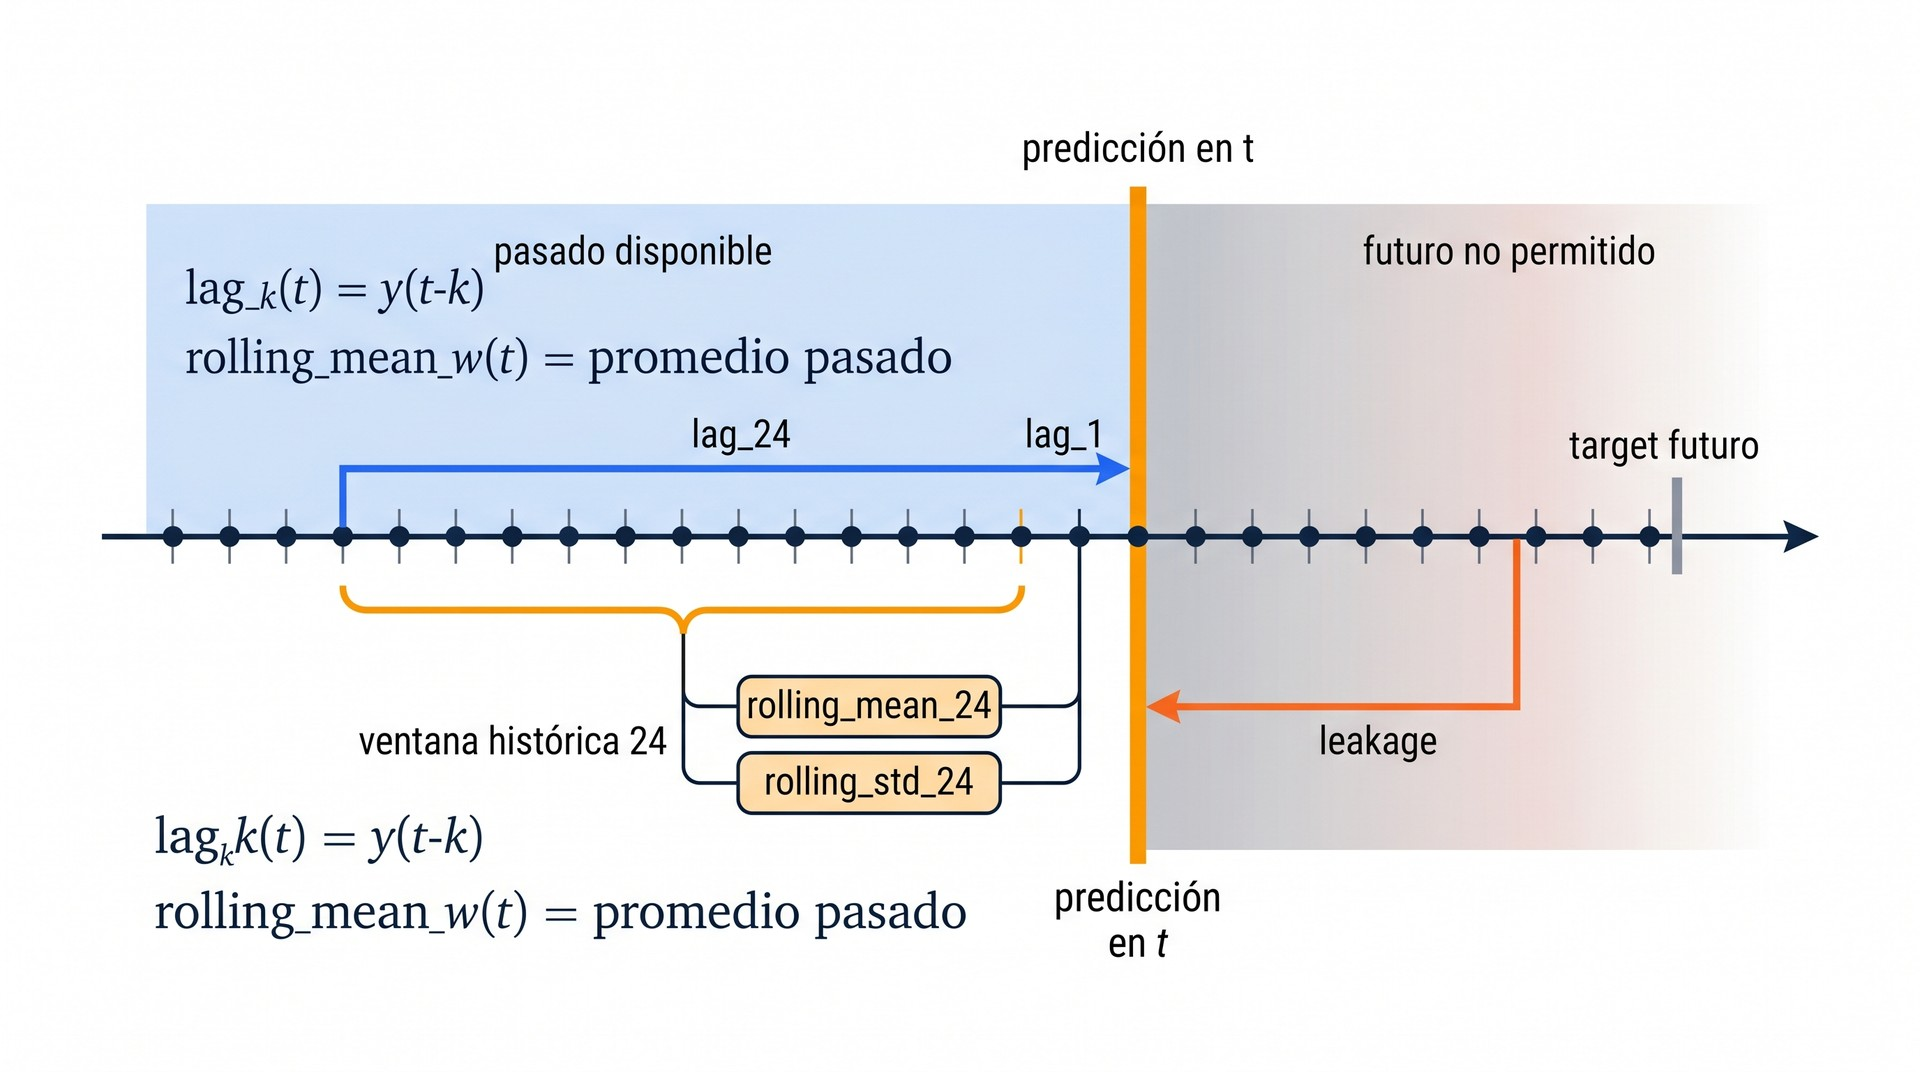
\includegraphics[width=\linewidth]{figures/img_p035_09.jpg}
\end{columns}
\begin{rulebox}[Leakage]
\small Una ventana que incluye $y_t$, $y_{t+1}$ o valores posteriores usa el futuro: el score mejora y en producción no se repite.
\end{rulebox}
\end{frame}

\begin{frame}{Feature temporal válida vs feature contaminada}
\framesubtitle{El nombre de la columna no garantiza la validez}
\centering\small
\begin{tabular}{@{}l P{0.36\textwidth} P{0.37\textwidth}@{}}
\toprule
\hrow \textbf{Feature} & Válida si\ldots & Contaminada si\ldots\\
\midrule
$\mathrm{lag}_1$ & usa un valor observado antes de predecir & se construye con el target futuro desplazado al revés\\
$\mathrm{lag}_{24}$ & representa la misma hora del día anterior disponible & usa una medición corregida después del periodo objetivo\\
$\mathrm{rolling\_mean}_{24}$ & promedia solo valores anteriores al momento $t$ & incluye $y_t$, $y_{t+1}$ o valores posteriores\\
clima & pronóstico disponible antes de las 8:00 AM & clima observado oficialmente a las 10:00 AM\\
\bottomrule
\end{tabular}
\raggedright
\begin{taskbox}[Práctica]
\small Para una predicción a las 8:00 AM, clasifique como válida, dudosa o contaminada: hora del día, festivo ya conocido, clima observado a las 10:00, pronóstico de las 7:00.
\end{taskbox}
\end{frame}

\begin{frame}{La hora no vive en una recta: vive en un ciclo}
\framesubtitle{El calendario es válido, pero debe codificarse como ciclo}
\begin{columns}[c]
\column{0.4\textwidth}
\[ \mathrm{hour}_{\sin} = \sin\!\left(\tfrac{2\pi\cdot \mathrm{hour}}{24}\right) \]
\[ \mathrm{hour}_{\cos} = \cos\!\left(\tfrac{2\pi\cdot \mathrm{hour}}{24}\right) \]
\begin{itemize}\small
\item \textbf{lineal}: 23 y 0 parecen muy distantes; frontera artificial en medianoche;
\item \textbf{cíclica}: cada hora es un punto del círculo; 23:00 y 00:00 quedan cerca;
\item hora, día, mes y festivos se conocen antes de predecir.
\end{itemize}
\column{0.58\textwidth}
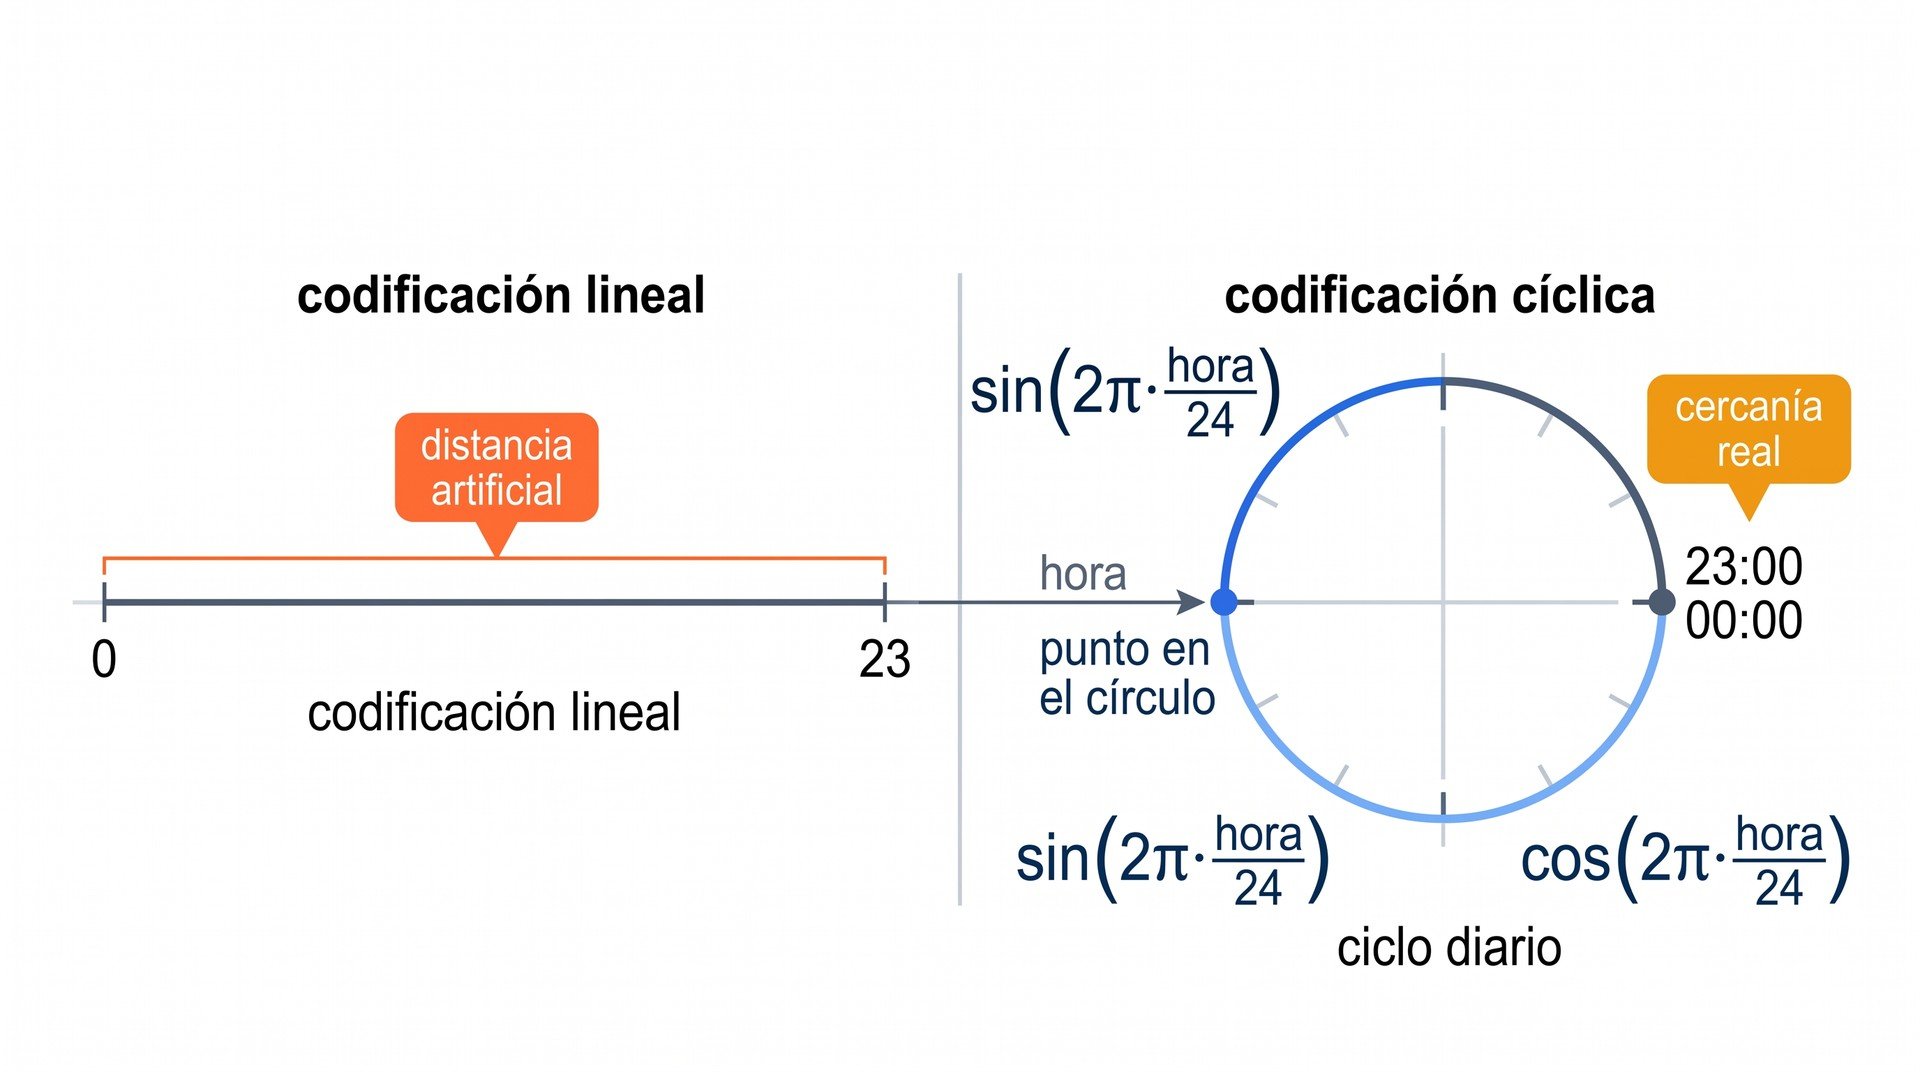
\includegraphics[width=\linewidth]{figures/img_p039_10.jpg}
\end{columns}
\vspace{2pt}
{\small Se necesitan las dos (seno \textbf{y} coseno): con una sola, horas distintas tendrían el mismo valor.\par}
\end{frame}

\begin{frame}{Codificación estacional: ciclos cortos y largos}
\framesubtitle{Seno/coseno, términos de Fourier y lags estacionales}
\centering\footnotesize
\begin{tabular}{@{}l P{0.30\textwidth} P{0.36\textwidth}@{}}
\toprule
\hrow \textbf{Variable} & Qué puede capturar & Codificación razonable\\
\midrule
\textbf{Hora del día} & ciclos de congestión o actividad & seno/coseno de 24 horas\\
\textbf{Día de la semana} & lunes frente a fin de semana & categórica o seno/coseno semanal\\
\textbf{Estacionalidad larga} & ciclo semanal (168 h) o anual & \textbf{Fourier}: $\sin\frac{2\pi k t}{s}$, $\cos\frac{2\pi k t}{s}$, $k = 1..K$\\
\textbf{Patrón exacto del ciclo} & la misma hora del ciclo anterior & \textbf{lag estacional} $y_{t-s}$\\
\textbf{Festivo} & cambios programados & indicador binario conocido antes de predecir\\
\bottomrule
\end{tabular}
\raggedright
\begin{keybox}[Cuándo usar cada uno]
\small Fourier con pocos $K$ describe ciclos largos con pocas columnas; el lag estacional copia la forma exacta del ciclo pero exige historia suficiente.
\end{keybox}
\end{frame}

% ============================================================ 6. modelos globales (G0-G3)
\section{Modelos globales}
\sectionframe{\LARGE De una serie a muchas:\\modelos globales}

\begin{frame}{Local frente a global}
\framesubtitle{Un modelo por serie o un modelo para todas las series}
\begin{columns}[T]
\column{0.48\textwidth}
\colhead{Modelo local}
\small Un modelo $f_j$ por cada serie $j$: 20 clientes $\rightarrow$ 20 modelos, cada uno con su propia historia.
\vspace{6pt}

\colhead{Modelo global}
\small Un solo $f$ entrenado con las filas de \textbf{todas} las series:
\[ \hat y_{j,t+h} = f\big(X_{j,t},\ \text{id}_j\big) \]
\column{0.48\textwidth}
\begin{goldbox}[Qué gana]
\small más datos por modelo · patrones compartidos (horas pico, festivos) · funciona con series nuevas o cortas.
\end{goldbox}
\begin{rulebox}[Qué arriesga]
\small series muy distintas entre sí · una serie grande domina la pérdida si no se escala · más difícil de depurar.
\end{rulebox}
\end{columns}
\end{frame}

\begin{frame}{Cómo se arma la tabla global}
\framesubtitle{Apilar series sin mezclar sus historias}
\centering
\begin{tikzpicture}[x=0.55cm,y=0.45cm]
  \foreach \j/\c in {0/eafitsky,1/mltealbg,2/mlcream}{
    \fill[\c] (0,-\j*1.3) rectangle ++(4,1); \node[font=\scriptsize] at (2,-\j*1.3+0.5) {serie \the\numexpr\j+1\relax};
    \fill[\c] (9,-\j*1.3) rectangle ++(6,1);
  }
  \node[font=\scriptsize] at (12,0.5) {filas de la serie 1};
  \node[font=\scriptsize] at (12,-0.8) {filas de la serie 2};
  \node[font=\scriptsize] at (12,-2.1) {filas de la serie 3};
  \draw[-{Stealth[length=2mm]},thick,eafitblue] (4.6,-0.8) -- (8.4,-0.8) node[midway,above,font=\tiny] {apilar};
\end{tikzpicture}
\par\vspace{4pt}
\raggedright\small
\begin{itemize}
\item columna \texttt{series\_id} y features estáticas de cada serie (tipo de cliente, región);
\item lags y rolling \textbf{por serie}: \texttt{df.groupby("series\_id")["y"].shift(1)};
\item \textbf{escalar por serie} (dividir por su media histórica, calculada solo en train) para que ninguna domine;
\item la identidad de la serie entra como categórica: el modelo puede aprender diferencias de nivel.
\end{itemize}
\end{frame}

\begin{frame}{Ejemplo: dos clientes, una sola tabla}
\framesubtitle{Consumo horario (kW), lags $L = 2$ y horizonte $h = 1$}
\centering\footnotesize
\begin{tabular}{@{}l *{5}{c}@{}}
\toprule
\hrow \textbf{hora} & 10:00 & 11:00 & 12:00 & 13:00 & 14:00\\
\midrule
cliente A (residencial) & 50 & 55 & 62 & 58 & 60\\
cliente B (comercial) & 400 & 420 & 480 & 470 & 450\\
\bottomrule
\end{tabular}
\par\vspace{1pt}
{\large$\Downarrow$}\ {\scriptsize apilar y calcular lags con \texttt{groupby("series\_id")}}
\par\vspace{1pt}
\begin{tabular}{@{}c l c >{\columncolor{eafitsky}}c >{\columncolor{eafitsky}}c >{\columncolor{mlredbg}}c@{}}
\toprule
\hrow \textbf{series\_id} & \textbf{tipo} & \textbf{hora $t$} & $y_{t-1}$ & $y_t$ & \textbf{target} $y_{t+1}$\\
\midrule
A & residencial & 11:00 & 50 & 55 & 62\\
A & residencial & 12:00 & 55 & 62 & 58\\
A & residencial & 13:00 & 62 & 58 & 60\\
\midrule
B & comercial & 11:00 & 400 & 420 & 480\\
B & comercial & 12:00 & 420 & 480 & 470\\
B & comercial & 13:00 & 480 & 470 & 450\\
\bottomrule
\end{tabular}
\par\vspace{3pt}
\raggedright\footnotesize
\begin{itemize}
\item un solo modelo aprende de las 6 filas; \texttt{series\_id} y \texttt{tipo} le dicen de qué serie viene cada una;
\item sin \texttt{groupby} aparecen filas falsas: B 10:00 con $y_{t-1} = 60$ y A 14:00 con target 400 (\textbf{mezcla de historias});
\item B está en otra escala (unas 8 veces A): sin escalar por serie, sus errores dominan la pérdida.
\end{itemize}
\end{frame}

\begin{frame}{Validar un modelo global}
\framesubtitle{El mismo protocolo temporal, aplicado a todas las series a la vez}
\begin{itemize}\small
\item walk-forward con el \textbf{mismo corte temporal} $T_k$ para todas las series;
\item nunca usar el futuro de una serie para predecir el pasado de otra;
\item el embargo $g$ se aplica igual en todas;
\item métricas \textbf{por serie} y agregadas (sección de métricas);
\item comparar contra modelos locales y contra el seasonal naïve de cada serie.
\end{itemize}
\begin{rulebox}[Leakage específico del modelo global]
\small Escalar cada serie con su media de \textbf{toda} la historia filtra el nivel futuro. La escala se calcula solo con el train de cada fold.
\end{rulebox}
\end{frame}

% ============================================================ 7. baselines (43, 44+46, 47+48)
\section{Baselines temporales}
\sectionframe{\LARGE Antes del modelo: demostrar que el\\pasado simple no basta}

\begin{frame}{Tres referencias temporales obligatorias}
\framesubtitle{Un baseline temporal no es un modelo ridículo}
\begin{columns}[c]
\column{0.38\textwidth}
\begin{itemize}\small
\item \textbf{Naïve} $\hat y_{t+h} = y_t$: aprovecha la \textbf{persistencia};
\item \textbf{Seasonal naïve} $\hat y_{t+h} = y_{t+h-s}$ ($s = 24$ en datos horarios): aprovecha el \textbf{ciclo};
\item \textbf{Moving average} $\hat y_{t+h} = \frac{1}{w}\sum_{i=0}^{w-1} y_{t-i}$: robusto con ruido local.
\end{itemize}
\column{0.6\textwidth}
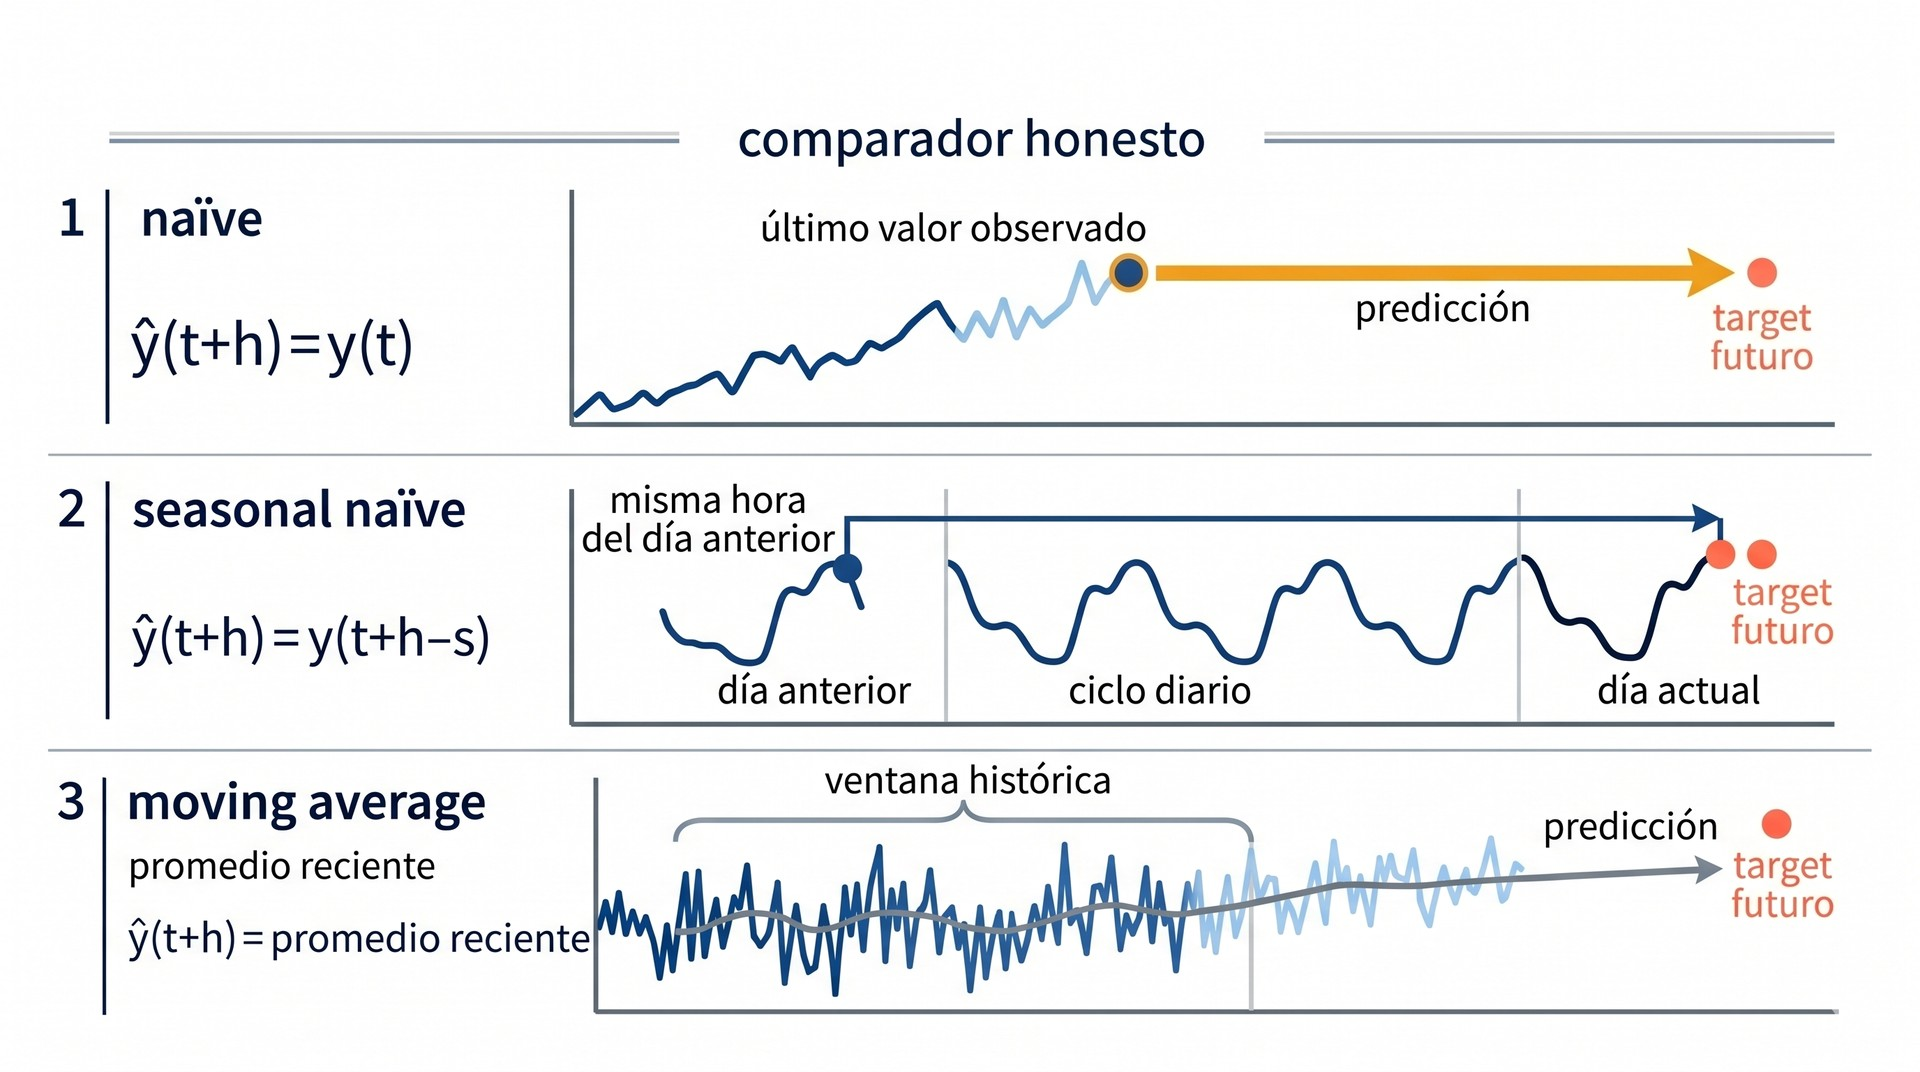
\includegraphics[width=\linewidth]{figures/img_p045_11.jpg}
\end{columns}
\begin{rulebox}[Criterio de clase]
\small Un modelo temporal sofisticado que no supera un baseline temporal honesto no merece una defensa fuerte.
\end{rulebox}
\end{frame}

\begin{frame}{Cuándo cada baseline pone presión real}
\framesubtitle{El baseline correcto depende de la estructura temporal dominante}
\centering\small
\begin{tabular}{@{}l P{0.35\textwidth} P{0.35\textwidth}@{}}
\toprule
\hrow \textbf{Baseline} & Es fuerte cuando\ldots & Puede fallar cuando\ldots\\
\midrule
\textbf{Naïve} & la serie tiene alta persistencia y cambia lentamente & hay cambios bruscos o ciclos fuertes\\
\textbf{Seasonal naïve} & existe patrón diario, semanal o mensual estable & el ciclo cambia por eventos, clima o régimen\\
\textbf{Moving average} & el nivel reciente resume bien el estado operativo & suaviza demasiado picos o eventos raros\\
\bottomrule
\end{tabular}
\raggedright
\begin{taskbox}[Práctica]
\small ¿Qué baseline usaría primero para: tráfico 1 hora adelante; demanda energética mañana a la misma hora; ventas diarias con fines de semana? En un modelo global, el baseline se calcula \textbf{por serie}.
\end{taskbox}
\end{frame}

% ============================================================ 8. validación temporal y leakage (49, 50+52+53, 56+57, 58+59, 60, 61, 62, 64+67, 66+68)
\section{Validación temporal y leakage}
\sectionframe{\LARGE Validación temporal:\\random split, walk-forward y leakage}

\begin{frame}{Random split puede ser una trampa temporal}
\framesubtitle{El futuro no debe entrenar el modelo que evalúa el pasado}
{\large\[ \exists\, t_i \in D_{\mathrm{train}},\ \exists\, t_j \in D_{\mathrm{val}} \ \text{tal que}\ t_i > t_j \]}
\centering\footnotesize
\begin{tabular}{@{}l P{0.34\textwidth} P{0.36\textwidth}@{}}
\toprule
\hrow \textbf{Esquema} & Qué hace & Riesgo o utilidad\\
\midrule
\textbf{Random split} & mezcla observaciones de distintos momentos & infla el desempeño si hay dependencia temporal\\
\textbf{Temporal holdout} & entrena en pasado y valida en un bloque futuro & simple, útil y más cercano a operación real\\
\textbf{Walk-forward} & repite la evaluación avanzando en el tiempo & estima desempeño de forma más robusta\\
\bottomrule
\end{tabular}
\raggedright
\begin{rulebox}[Regla]
\small El score puede subir no porque el modelo sea mejor, sino porque el experimento fue más fácil. El split debe responder: ¿cómo habría funcionado el modelo si se hubiera usado en ese momento?
\end{rulebox}
\end{frame}

\begin{frame}{Validar hacia adelante}
\framesubtitle{Entrenar con pasado, validar en futuro y repetir}
\begin{columns}[c]
\column{0.44\textwidth}
\begin{itemize}\small
\item el modelo se entrena con historia disponible;
\item predice un bloque futuro;
\item el origen de predicción avanza;
\item el desempeño se resume sobre varios bloques.
\end{itemize}
\vspace{4pt}
{\small La validación temporal pregunta: ¿qué habría pasado si el modelo se hubiera usado en ese momento?\par}
\column{0.52\textwidth}
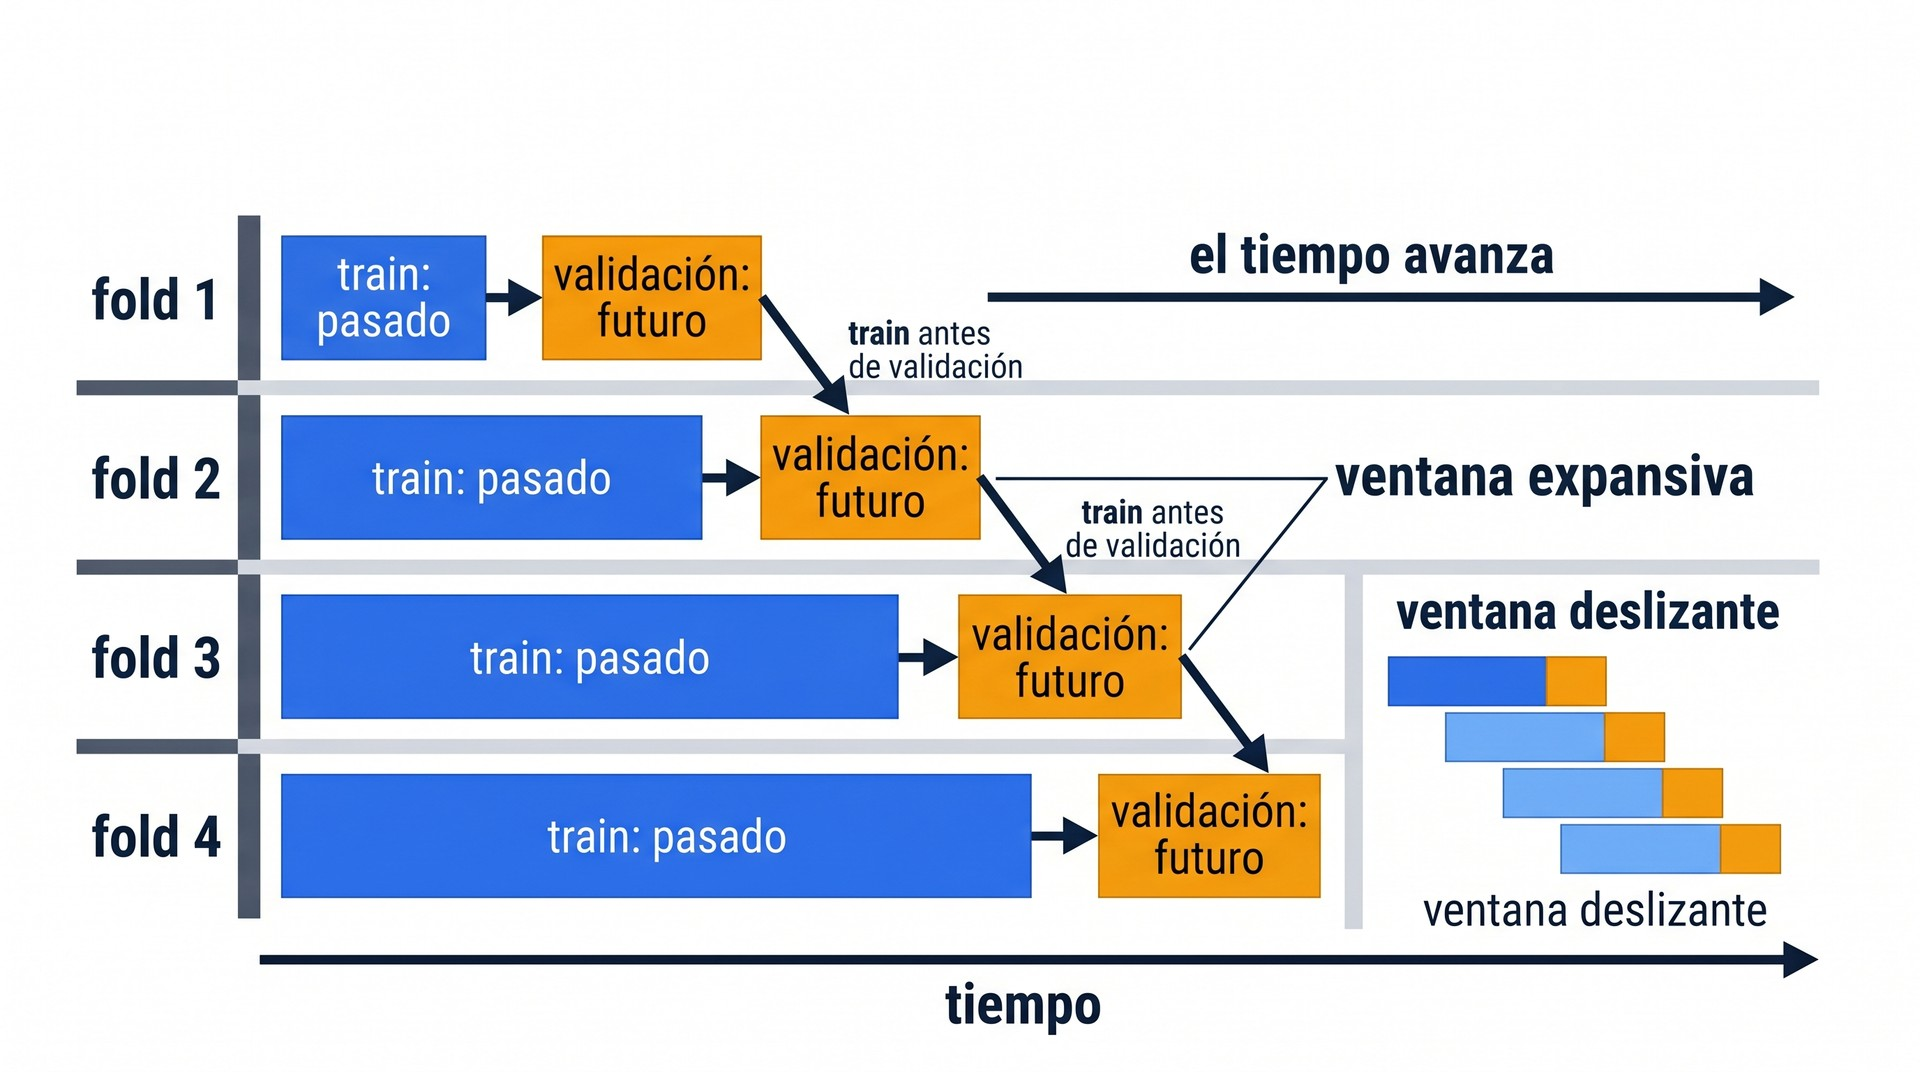
\includegraphics[width=\linewidth]{figures/img_p057_13.jpg}
\end{columns}
\end{frame}

\begin{frame}{La restricción cronológica y el score final}
\framesubtitle{Cada validación debe estar después de su entrenamiento}
\begin{gather*}
D^{(k)}_{\mathrm{train}} = \bigl\{(X_t, y_{t+h}) : t \le T_k\bigr\} \qquad D^{(k)}_{\mathrm{val}} = \bigl\{(X_t, y_{t+h}) : T_k < t \le T_{k+1}\bigr\}\\[0.4em]
\max\Bigl(t \in D^{(k)}_{\mathrm{train}}\Bigr) < \min\Bigl(t \in D^{(k)}_{\mathrm{val}}\Bigr)
\qquad\qquad
\widehat{E}_{\mathrm{WF}} = \frac{1}{K}\sum_{k=1}^{K} E\Bigl(D^{(k)}_{\mathrm{val}}\Bigr)
\end{gather*}
\begin{itemize}\small
\item en cada fold, el entrenamiento termina antes de que empiece la validación;
\item $K$: número de cortes; $E(D^{(k)}_{\mathrm{val}})$: error del fold $k$ en un bloque futuro;
\item el score final promedia varios futuros evaluados, no una medición aislada (reporte también la dispersión).
\end{itemize}
\end{frame}

\begin{frame}{Variantes útiles de validación temporal}
\framesubtitle{La decisión depende de historia disponible, estabilidad y costo computacional}
\centering
\begin{tabular}{@{}l P{0.33\textwidth} P{0.33\textwidth}@{}}
\toprule
\hrow \textbf{Esquema} & Cómo entrena & Cuándo tiene sentido\\
\midrule
\textbf{Holdout temporal} & un bloque pasado para train y un bloque futuro para validación & primera comparación simple y clara\\
\textbf{Ventana expansiva} & cada fold acumula más historia antes de validar el siguiente bloque & cuando más historia suele aportar señal útil\\
\textbf{Ventana deslizante} & cada fold usa solo una ventana reciente de longitud fija & cuando los patrones antiguos dejan de representar el presente\\
\bottomrule
\end{tabular}

\vspace{0.4em}
No existe una única validación temporal universal: debe corresponder al uso real, al horizonte y a la estabilidad del fenómeno.
\end{frame}

\begin{frame}[fragile]{Embargo: una separación cuando hay riesgo de vecindad}
\framesubtitle{No todo fold cronológico queda automáticamente limpio}
{\large\[ \max(t_{\mathrm{train}}) + g < \min(t_{\mathrm{val}}) \]}
\begin{columns}[T]
\column{0.48\textwidth}
\begin{itemize}\small
\item $g$: tamaño de la brecha temporal;
\item $g = 24$ en datos horarios deja un día de separación;
\item útil si las features usan ventanas largas o labels futuros;
\item no reemplaza una mala formulación.
\end{itemize}
\column{0.48\textwidth}
\begin{lstlisting}[language=Python,basicstyle=\ttfamily\scriptsize,numbers=none]
from sklearn.model_selection import TimeSeriesSplit
tscv = TimeSeriesSplit(n_splits=5,
                       test_size=24 * 28,
                       gap=24)     # embargo
\end{lstlisting}
{\footnotesize Es la CV temporal de la S1, ahora con embargo.\par}
\end{columns}
\end{frame}

\begin{frame}{Práctica: diseñe el protocolo}
\framesubtitle{El split debe ser una decisión defendible, no una línea de código por costumbre}
\begin{taskbox}[{\large Escenario}]
Datos horarios de tráfico entre 2012 y 2018. Quiere predecir una hora adelante y comparar seasonal naïve, Ridge e HistGradientBoostingRegressor.
\end{taskbox}
\textbf{Defina:}
\begin{enumerate}\small
\item tamaño del bloque inicial de entrenamiento y del bloque de validación;
\item ventana expansiva o deslizante, y si necesita embargo;
\item qué métrica reportaría por fold y cómo resumiría el desempeño final;
\item cómo cambia el protocolo si son 20 clientes de electricidad (modelo global).
\end{enumerate}
\end{frame}

\begin{frame}{Leakage temporal: la regla formal}
\framesubtitle{La pregunta no es ``¿la columna existe?'', sino ``¿el sistema la conocía antes de predecir?''}
\begin{align*}
x_j(t) \in \mathcal{I}_t \quad &\Longrightarrow \quad x_j(t) \text{ es candidata válida}\\[0.4em]
x_j(t) \notin \mathcal{I}_t \quad &\Longrightarrow \quad x_j(t) \text{ introduce riesgo de leakage}
\end{align*}
\begin{defbox}[$\mathcal{I}_t$]
\small Conjunto de información que el sistema podía conocer antes o en el momento operativo de predicción $t$.
\end{defbox}
\small El leakage puede entrar por features que miran hacia adelante, preprocessing ajustado con toda la serie, variables externas publicadas tarde o folds que mezclan futuro y pasado.
\end{frame}

\begin{frame}{Rutas comunes de leakage temporal}
\framesubtitle{El futuro puede entrar por features, preprocessing o validación}
\centering\footnotesize
\begin{tabular}{@{}P{0.25\textwidth} P{0.32\textwidth} P{0.32\textwidth}@{}}
\toprule
\hrow \textbf{Ruta} & Qué parece hacer & Por qué contamina\\
\midrule
\textbf{Rolling mal alineado} & calcula una media móvil suave & incluye $y_t$, $y_{t+1}$ o valores posteriores\\
\textbf{Escalamiento global} & normaliza todas las filas antes del split & aprende estadísticas del futuro\\
\textbf{Escala por serie con toda la historia} & normaliza cada serie del modelo global & filtra el nivel futuro de cada serie\\
\textbf{Variable externa tardía} & agrega clima o evento observado después & la señal no existía al decidir\\
\textbf{Folds mezclados} & valida en pasado y entrena con futuro & rompe la dirección operacional\\
\bottomrule
\end{tabular}
\raggedright
\begin{taskbox}[Práctica: audite]
\footnotesize ¿Qué falla en: \texttt{rolling\_mean}$_{24}$ con ventana centrada; \texttt{StandardScaler} ajustado con todo el histórico; features elegidas mirando el bloque de test?
\end{taskbox}
\end{frame}

% ============================================================ 9. métricas y multi-horizonte (69, 71+70, 73+74, 75+76, M1, 78+79+80, 81+82)
\section{Métricas y multi-horizonte}
\sectionframe{\LARGE Medir error no basta: hay que\\interpretarlo contra tiempo y baseline}

\begin{frame}{MAE y RMSE: dos lecturas del error}
\framesubtitle{El error se lee contra un baseline y un horizonte}
\begin{columns}[T]
\column{0.47\textwidth}
{\large\[ \mathrm{MAE} = \frac{1}{n}\sum_{i=1}^{n} |y_i - \hat y_i| \]}
\begin{itemize}\small
\item en unidades del target;
\item fácil de comunicar;
\item resume el error típico absoluto.
\end{itemize}
\column{0.49\textwidth}
{\large\[ \mathrm{RMSE} = \sqrt{\frac{1}{n}\sum_{i=1}^{n} (y_i - \hat y_i)^2} \]}
\begin{itemize}\small
\item castiga más los errores grandes;
\item sensible a picos;
\item útil si los desvíos extremos son costosos.
\end{itemize}
\end{columns}
\begin{rulebox}[Cuidado]
\small Un MAE aparentemente bajo puede ser mediocre si el seasonal naïve logra lo mismo con una regla simple.
\end{rulebox}
\end{frame}

\begin{frame}{MASE: escalar el error con una referencia temporal}
\framesubtitle{La pregunta es: ¿mejoro una predicción naïve?}
{\large\[ \mathrm{MASE} = \frac{\frac{1}{n}\sum_{i=1}^{n} |y_i - \hat y_i|}{\frac{1}{T_{\mathrm{train}}-m}\sum_{t=m+1}^{T_{\mathrm{train}}} |y_t - y_{t-m}|} \]}
\begin{columns}[T]
\column{0.5\textwidth}
\begin{itemize}\small
\item numerador: error absoluto medio del modelo;
\item denominador: error del naïve ($m = 1$) o del seasonal naïve ($m = 24$) \textbf{en train};
\item no depende de la escala: sirve para comparar series.
\end{itemize}
\column{0.46\textwidth}
\centering\small
\begin{tabular}{@{}c l@{}}
\toprule
\hrow \textbf{Valor} & Interpretación\\
\midrule
$< 1$ & mejora al baseline\\
$\approx 1$ & similar al baseline\\
$> 1$ & peor que el baseline\\
\bottomrule
\end{tabular}
\end{columns}
\end{frame}

\begin{frame}{MAPE, sMAPE y WAPE: alternativas con cautela}
\framesubtitle{El porcentaje parece intuitivo y aun así puede engañar}
\begin{columns}[T]
\column{0.5\textwidth}
\begin{itemize}\small
\item \textbf{MAPE} divide por el valor real: si es bajo o cercano a cero, explota;
\item \textbf{sMAPE} lo simetriza dividiendo por el promedio de real y predicción, pero sigue siendo inestable cerca de cero:
\end{itemize}
\[ \mathrm{sMAPE} = \frac{1}{n}\sum_i \frac{|y_i - \hat y_i|}{\big(|y_i| + |\hat y_i|\big)/2} \]
\begin{itemize}\small
\item \textbf{WAPE} divide el error total por el volumen total:
\end{itemize}
\[ \mathrm{WAPE} = \frac{\sum_i |y_i - \hat y_i|}{\sum_i |y_i|} \]
\column{0.46\textwidth}
\begin{taskbox}[Práctica]
\small ¿Qué métrica principal para: tráfico (error típico en vehículos), energía (errores extremos costosos), inventario (superar al naïve)?
\end{taskbox}
\begin{goldbox}[Regla de la sesión]
\small MAE, RMSE y MASE son centrales; WAPE para agregados con ceros.
\end{goldbox}
\end{columns}
\end{frame}

\begin{frame}{Métricas para muchas series}
\framesubtitle{Un modelo global se evalúa por serie y en conjunto}
\centering\small
\begin{tabular}{@{}l P{0.34\textwidth} P{0.36\textwidth}@{}}
\toprule
\hrow \textbf{Métrica} & Cómo se calcula & Qué pregunta responde\\
\midrule
\textbf{MAE promedio} & MAE de cada serie y su media & engañosa: las series grandes dominan\\
\textbf{MASE promedio} & MASE de cada serie (escala propia) y su media & ¿el modelo mejora al naïve en una serie típica?\\
\textbf{WAPE agregado} & error total / volumen total de todas las series & ¿cuánto volumen total se predice mal?\\
\textbf{RMSSE} & raíz del error cuadrático escalado por el naïve (M5) & como MASE, pero castiga errores grandes\\
\bottomrule
\end{tabular}
\raggedright
\begin{keybox}[Lectura]
\small No se promedian errores de series con escalas distintas sin escalarlos primero. Reporte también cuántas series mejoran al baseline.
\end{keybox}
\end{frame}

\begin{frame}{Un modelo no tiene un único desempeño temporal}
\framesubtitle{El error debe indexarse por la distancia al futuro}
\begin{columns}[c]
\column{0.5\textwidth}
\[ \widehat{y}_{t+h} = f_h(X_t) \qquad h \in \{1, 3, 6, 24\} \]
\[ E_h = \frac{1}{n_h}\sum_{i=1}^{n_h} L(y_{t_i+h}, \widehat{y}_{t_i+h}) \]
\begin{itemize}\small
\item horizonte corto: domina el estado reciente y los lags cercanos;
\item horizonte largo: más incertidumbre; dominan ciclos y calendario.
\end{itemize}
\column{0.46\textwidth}
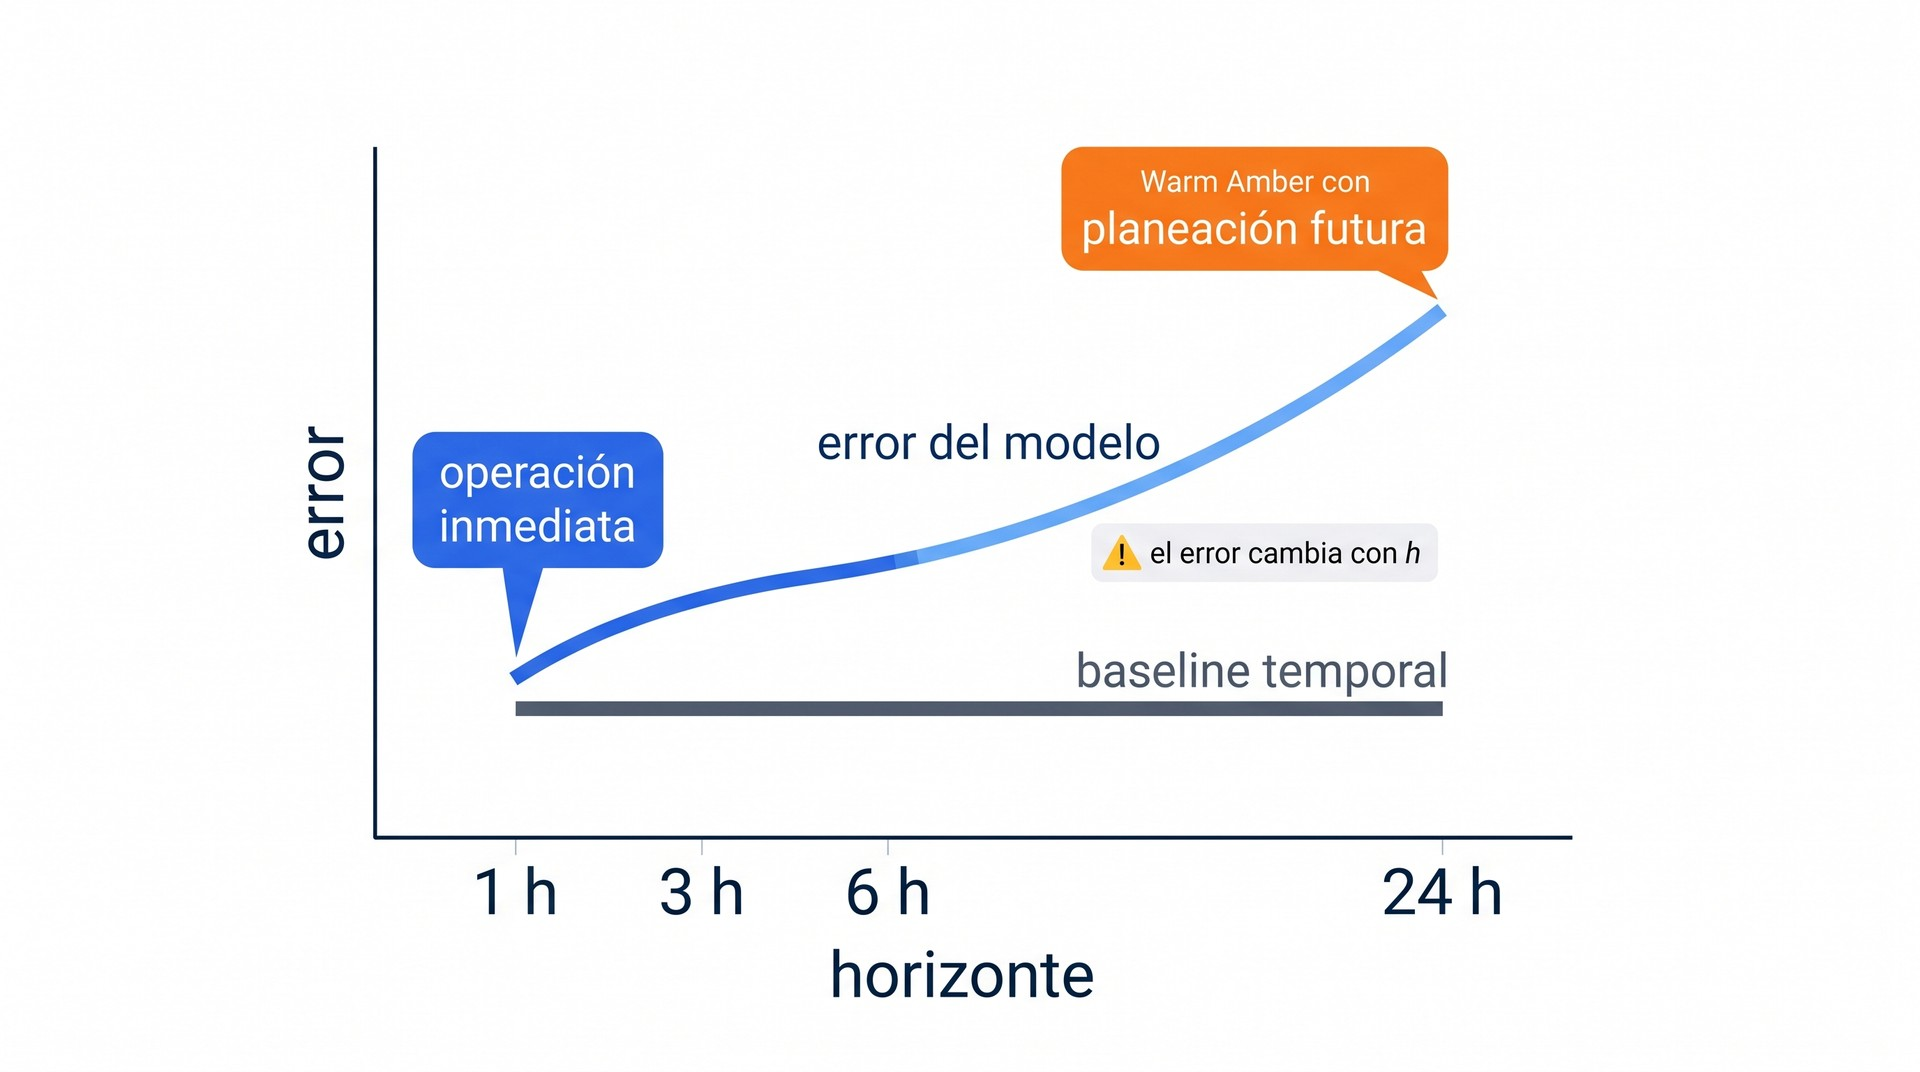
\includegraphics[width=\linewidth]{figures/img_p079_16.jpg}
\end{columns}
\end{frame}

\begin{frame}{Cómo cambia la utilidad por horizonte}
\framesubtitle{La métrica debe leerse con la decisión que habilita}
\centering\small
\begin{tabular}{@{}l P{0.39\textwidth} P{0.40\textwidth}@{}}
\toprule
\hrow \textbf{Horizonte} & Señal que suele dominar & Decisión que puede soportar\\
\midrule
\textbf{1 hora} & estado reciente, $\mathrm{lag}_1$, tendencia local & gestión inmediata de congestión o alertas\\
\textbf{6 horas} & ciclos diarios parciales y contexto externo & anticipación de carga en media jornada\\
\textbf{24 horas} & estacionalidad diaria, calendario, patrones recurrentes & planeación del día siguiente\\
\bottomrule
\end{tabular}
\raggedright
\begin{taskbox}[Práctica]
\small El modelo A gana en MAE a 1 hora; el B es más estable a 6 y 24 horas. El equipo necesita planear el día siguiente: ¿cuál defiende y qué baseline debe aparecer?
\end{taskbox}
\end{frame}

% ============================================================ 10. modelos, notebook y demo (83, 84+85, O1, 99+100+97, 102+104, H1)
\section{Modelos, notebook y demo}
\sectionframe{\LARGE El modelo entra cuando el\\experimento ya es defendible}

\begin{frame}{Primero formulación, después complejidad}
\framesubtitle{Los modelos compiten contra baselines bajo el mismo protocolo temporal}
\begin{columns}[T]
\column{0.32\textwidth}
\textbf{Antes del modelo}
\begin{itemize}\small
\item target y horizonte;
\item features válidas;
\item baselines temporales;
\item walk-forward.
\end{itemize}
\column{0.64\textwidth}
\centering\footnotesize
\begin{tabular}{@{}l P{0.6\linewidth}@{}}
\toprule
\hrow \textbf{Modelo} & Papel\\
\midrule
\textbf{Ridge} & referencia supervisada lineal, fácil de explicar\\
\textbf{HistGradientBoosting} & no linealidad e interacciones (Metro)\\
\textbf{HGBR o LightGBM global} & un solo modelo para muchas series (Electricity)\\
\bottomrule
\end{tabular}
\end{columns}
\begin{rulebox}[Después del modelo]
\small Si el modelo gana, debe ganar contra una referencia honesta, sin leakage y en el horizonte que importa.
\end{rulebox}
\end{frame}

\begin{frame}{Familias de modelos temporales}
\framesubtitle{De más supuestos a más flexibilidad, bajo la misma validación}
\centering
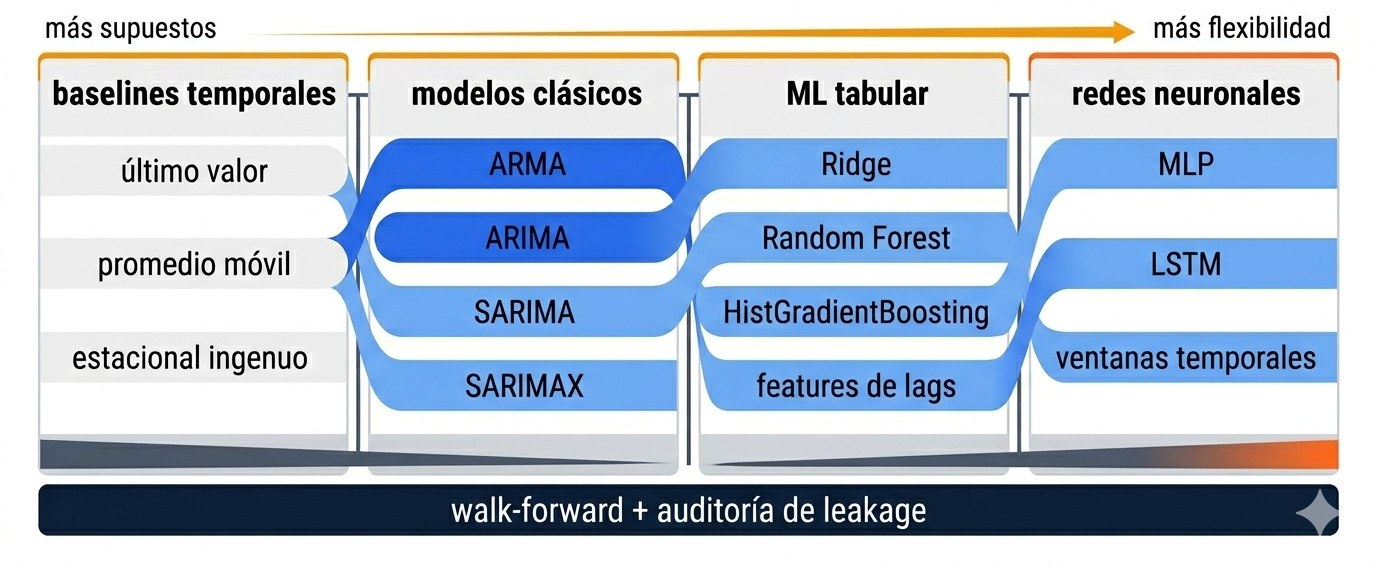
\includegraphics[width=0.7\textwidth]{figures/img_p088_18_crop.jpg}
\par\vspace{2pt}\raggedright\footnotesize
\begin{itemize}
\item \textbf{clásicos} (ARIMA, SARIMA, SARIMAX): pocos parámetros, una serie a la vez, estructura explícita;
\item \textbf{ML tabular}: la memoria entra como features (lags, rolling, calendario); escala a modelos globales;
\item todos se comparan con el mismo target, horizonte, baseline y walk-forward.
\end{itemize}
\end{frame}

\begin{frame}{ARIMA$(p,d,q)$: valores, cambios y errores pasados}
\framesubtitle{Un modelo lineal sobre la propia historia de la serie}
\begin{columns}[c]
\column{0.44\textwidth}
\small Sobre la serie diferenciada $y'_t = \nabla^d y_t$:
\[ y'_t = c + \underbrace{\sum_{i=1}^{p} \phi_i\, y'_{t-i}}_{\text{AR: valores}} + \underbrace{\sum_{j=1}^{q} \theta_j\, \varepsilon_{t-j}}_{\text{MA: errores}} + \varepsilon_t \]
\begin{itemize}\small
\item $p$: lags de la serie (orienta la PACF);
\item $d$: diferencias para quitar tendencia;
\item $q$: errores pasados que corrigen (orienta la ACF).
\end{itemize}
\column{0.54\textwidth}
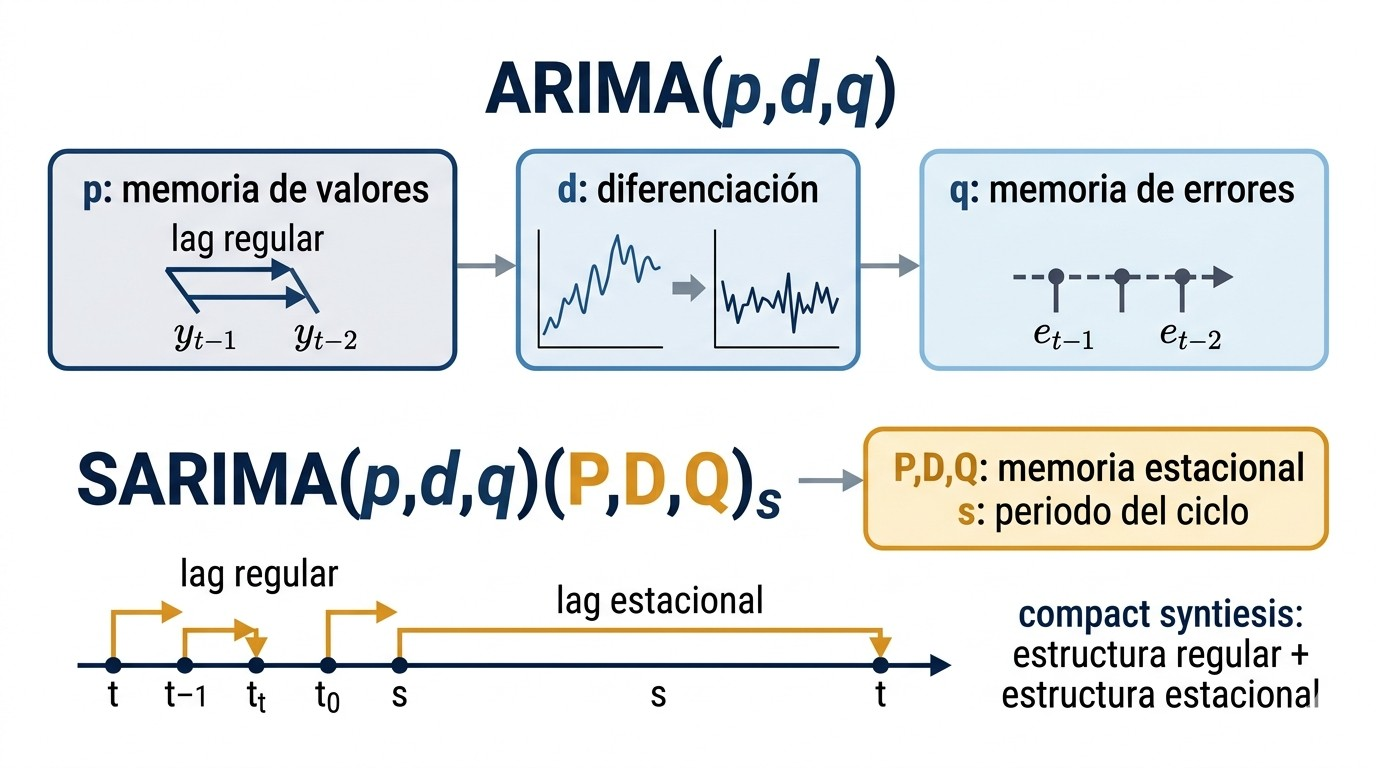
\includegraphics[width=\linewidth]{figures/img_p090_19.jpg}
\end{columns}
\vspace{2pt}
{\small\textbf{Conexión:} la parte AR es una regresión lineal sobre lags, como Ridge con \texttt{lag\_1}, \ldots, \texttt{lag\_p}.\par}
\end{frame}

\begin{frame}{SARIMA y SARIMAX: ciclo y variables externas}
\framesubtitle{$\text{SARIMA}(p,d,q)(P,D,Q)_s$ y la versión con exógenas}
\begin{columns}[T]
\column{0.48\textwidth}
\colhead{SARIMA: agrega el ciclo}
\begin{itemize}\small
\item $(P,D,Q)$ repiten la idea de ARIMA con lags \textbf{estacionales} $y_{t-s}, y_{t-2s}, \ldots$;
\item $s$: periodo del ciclo ($s = 24$ en datos horarios con ciclo diario);
\item ejemplo: $(1,0,1)(1,1,1)_{24}$ usa la hora anterior y la misma hora de ayer.
\end{itemize}
\column{0.48\textwidth}
\colhead{SARIMAX: agrega exógenas}
\[ y_t = \beta^\top x_t + \text{SARIMA}(\ldots) \]
\begin{itemize}\small
\item $x_t$: clima, festivos, precio, promociones;
\item para predecir $t+h$ se necesita $x_{t+h}$: solo vale si se \textbf{conoce} (festivo) o se usa su \textbf{pronóstico} (clima).
\end{itemize}
\end{columns}
\vspace{2pt}
\begin{rulebox}[Leakage en SARIMAX]
\small Usar el clima \textbf{observado} de mañana en lugar del pronosticado da un score que en producción no existe.
\end{rulebox}
\end{frame}

\begin{frame}{Clásico frente a ML tabular}
\framesubtitle{Cuándo probar cada uno}
\centering\small
\begin{tabular}{@{}l P{0.36\textwidth} P{0.36\textwidth}@{}}
\toprule
\hrow & \textbf{ARIMA / SARIMA(X)} & \textbf{ML tabular (HGBR, LightGBM)}\\
\midrule
\textbf{Memoria} & órdenes $p, q, P, Q$ & lags y rolling como columnas\\
\textbf{Estacionalidad} & $(P,D,Q)_s$, un solo periodo & calendario, Fourier, varios ciclos a la vez\\
\textbf{Exógenas} & lineales ($\beta^\top x_t$) & no lineales e interacciones\\
\textbf{Muchas series} & un modelo por serie (local) & un modelo global\\
\textbf{Datos} & funciona con historias cortas & necesita más filas\\
\textbf{Salida} & intervalos de predicción nativos & puntual (intervalos con quantile loss)\\
\bottomrule
\end{tabular}
\raggedright\par\vspace{4pt}
\small En \texttt{statsmodels}: \texttt{SARIMAX(y, exog=X, order=(p,d,q), seasonal\_order=(P,D,Q,s))}. Se evalúa con el \textbf{mismo} walk-forward y MASE que el resto.
\end{frame}

\begin{frame}[fragile]{El notebook ejecuta el contrato metodológico}
\framesubtitle{Pseudocódigo y qué debe inspeccionarse}
\begin{columns}[T]
\column{0.46\textwidth}
\begin{lstlisting}[basicstyle=\ttfamily\scriptsize,numbers=left,numberstyle=\tiny\color{mlgray},commentstyle=\color{mltext}\itshape]
# 1. Ordenar por tiempo (y por serie)
# 2. Target futuro: y.shift(-h)
# 3. Lags: y.shift(k) por serie
# 4. Rolling: y.shift(1).rolling(w)
# 5. Split cronológico + embargo
# 6. Preprocessing solo en train
# 7. Métricas por fold y horizonte
\end{lstlisting}
\column{0.5\textwidth}
\centering\footnotesize
\begin{tabular}{@{}l P{0.55\linewidth}@{}}
\toprule
\hrow \textbf{Salida} & Pregunta\\
\midrule
Dummy manual & ¿se ve la alineación lag--target?\\
Serie sintética & ¿random split infla el score?\\
Baselines & ¿el modelo los supera?\\
Walk-forward & ¿es estable entre folds?\\
Multi-horizonte & ¿cómo se degrada el error?\\
Global vs local & ¿mejoran MASE y WAPE por serie?\\
\bottomrule
\end{tabular}
\end{columns}
\end{frame}

\begin{frame}{La historia aplicada de la demo}
\framesubtitle{El resultado cambia cuando cambia el protocolo de validación}
\begin{columns}[T]
\column{0.5\textwidth}
\centering\footnotesize
\begin{tabular}{@{}l P{0.55\linewidth}@{}}
\toprule
\hrow \textbf{Componente} & Decisión\\
\midrule
Target & volumen de tráfico futuro\\
Horizontes & $h = 1$; también $3, 6, 24$\\
Features & lags, rolling, calendario, clima disponible\\
Baselines & naïve, seasonal naïve, MA\\
Modelos & Ridge e HGBR\\
Validación & holdout temporal y walk-forward\\
\bottomrule
\end{tabular}
\column{0.46\textwidth}
\textbf{La demo debe mostrar}
\begin{enumerate}\small
\item random split como anti-ejemplo;
\item holdout temporal como primera corrección;
\item walk-forward como evaluación operacional;
\item baselines antes de modelos;
\item error por horizonte antes de concluir.
\end{enumerate}
\end{columns}
\end{frame}

\begin{frame}{Hands-on de la sesión}
\framesubtitle{Los tres ejercicios del syllabus}
\begin{enumerate}
\item \textbf{Modelo global}: un HGBR o LightGBM para ~20 clientes de electricidad frente a modelos locales y al seasonal naïve de cada serie (MASE y WAPE por serie).
\item \textbf{Walk-forward}: protocolo con ventana expansiva y embargo sobre Metro; dispersión del error entre folds.
\item \textbf{Comparar horizontes}: MAE y MASE para $h \in \{1, 3, 6, 24\}$; ¿dónde gana cada modelo?
\end{enumerate}
\vspace{4pt}
\begin{toolbox}[Notebook]
\href{https://github.com/anvasquezre/EAFIT_AA_2026-02/blob/main/notebooks/03_ml_time_series_walkforward.ipynb}{\textcolor{eafitneon}{\underline{\texttt{03\_ml\_time\_series\_walkforward.ipynb}}}} (local con \texttt{uv} o en Colab) · sección de modelo global: \pend{por publicar}
\end{toolbox}
\end{frame}

% ============================================================ 11. cierre (105, 107+111+117, 109, O2, 116+115, 118, 119)
\section{Cierre}
\sectionframe{\LARGE Checklist temporal y cierre\\metodológico}

\begin{frame}{Un resultado temporal defendible es una cadena}
\framesubtitle{Si falta un eslabón, el score pierde credibilidad}
\begin{columns}[T]
\column{0.47\textwidth}
\textbf{Evidencia fuerte}
\begin{itemize}\small
\item target y horizonte explícitos;
\item features disponibles en $t$;
\item baseline temporal superado;
\item walk-forward sin contaminación;
\item error reportado por horizonte.
\end{itemize}
\column{0.47\textwidth}
\textbf{Evidencia frágil}
\begin{itemize}\small
\item random split sin justificación;
\item rolling windows mal alineadas;
\item preprocessing antes del split;
\item un único score para todos los horizontes.
\end{itemize}
\end{columns}
\begin{keybox}[Lo que debe quedar claro]
\small Si el problema tiene tiempo, el futuro no puede ayudar a entrenar, transformar, seleccionar o validar el pasado.
\end{keybox}
\end{frame}

\begin{frame}{Glosario}
\framesubtitle{Términos que deben usarse con precisión}
\centering\scriptsize
\begin{tabular}{@{}l P{0.66\textwidth}@{}}
\toprule
\hrow \textbf{Término} & Interpretación operativa\\
\midrule
\textbf{Momento $t$ / horizonte $h$} & instante de decisión / distancia al target futuro\\
\textbf{Lag / rolling window} & memoria puntual / resumen de una ventana que mira solo hacia atrás\\
\textbf{Ventana deslizante} & fila formada por los últimos $L$ valores y un objetivo $h$ pasos adelante\\
\textbf{Directa / recursiva} & un modelo por horizonte / un modelo a 1 paso que se realimenta\\
\textbf{Fourier} & pares seno/coseno para estacionalidades largas\\
\textbf{Modelo global} & un modelo entrenado con muchas series a la vez\\
\textbf{Walk-forward / embargo} & validación que avanza en el tiempo / brecha $g$ entre train y validación\\
\textbf{MASE / WAPE / RMSSE} & error relativo al naïve / error total sobre volumen / MASE cuadrático\\
\bottomrule
\end{tabular}
\end{frame}

\begin{frame}{(Opcional) Estabilidad y diferenciación}
\framesubtitle{Cuándo el pasado representa el futuro y cómo trabajar con cambios}
{\large\[ \nabla y_t = y_t - y_{t-1} \qquad\qquad \nabla_s y_t = y_t - y_{t-s} \]}
\begin{columns}[T]
\column{0.47\textwidth}
\textbf{Estacionariedad (criterio práctico)}
\begin{itemize}\small
\item ¿pasado y futuro tienen una estructura comparable?
\item si la media cambia mucho, el pasado representa mal el futuro;
\item no se asume: se inspecciona y se valida hacia adelante.
\end{itemize}
\column{0.47\textwidth}
\textbf{Diferenciación}
\begin{itemize}\small
\item regular: reduce tendencia ($d$ en ARIMA);
\item estacional: reduce ciclos repetidos ($D$ en SARIMA);
\item el modelo aprende variaciones, no valores absolutos.
\end{itemize}
\end{columns}
\end{frame}

\begin{frame}{Preguntas de revisión para examen, taller y PI}
\framesubtitle{La evaluación buscará decisiones correctas, no trivia de librerías}
\begin{columns}[T]
\column{0.5\textwidth}
\begin{enumerate}\small
\item ¿Cuál es el target temporal y el horizonte?
\item ¿Qué features existían en el momento $t$?
\item ¿Qué baseline temporal debe ser superado?
\item ¿Qué split respeta la cronología? ¿Necesita embargo?
\item ¿Dónde podría entrar leakage antes del modelo?
\end{enumerate}
\column{0.46\textwidth}
\begin{enumerate}\small\setcounter{enumi}{5}
\item ¿Directa o recursiva para 24 pasos?
\item ¿Cuándo un modelo global en vez de uno por serie?
\item ¿Por qué no promediar MAE entre series?
\item ¿El error se reporta por horizonte?
\end{enumerate}
\end{columns}
\vspace{4pt}
{\small En el taller: el código que corre no basta; la evaluación debe sostener una decisión.\par}
\end{frame}

\begin{frame}{Transición a la siguiente sesión}
\framesubtitle{Después del tiempo aparecen usuarios, ítems, interacciones y rankings}
\begin{center}\large
Hoy rompimos la idea de que las filas son intercambiables cuando existe tiempo.\\[0.8em]
En la próxima sesión, romperemos otra intuición: no siempre queremos predecir un único valor, a veces queremos ordenar opciones para una persona.
\end{center}
\begin{keybox}[Sesión 4]
\small Recomendadores (matriz de utilidad, feedback implícito, ALS, híbridos) e interpretabilidad con SHAP.
\end{keybox}
\end{frame}

\begin{frame}[plain]
\begin{tikzpicture}[remember picture,overlay]
\node[anchor=north west,inner sep=0] at ([xshift=309bp,yshift=-45bp]current page.north west)
  {
\includegraphics[width=117bp,height=78bp]{figures/img_p119_28.jpg}};
\node[anchor=north west,inner sep=0] at ([xshift=177bp,yshift=-191bp]current page.north west)
  {
\includegraphics[width=96bp,height=64bp]{figures/img_p119_29.jpg}};
\node[anchor=center,align=center] at ([xshift=160bp,yshift=-86bp]current page.north west)
  {{\color{mltitle}\huge\bfseries Gracias por su atención}\\[0.5em]
   {\color{mltitle}\large ¿Preguntas, comentarios o discusión?}};
\node[anchor=center,align=center,font=\small] at ([xshift=227bp,yshift=-165bp]current page.north west)
  {\textbf{Aprendizaje Automático}\\
   SI7009 · Universidad EAFIT};
\end{tikzpicture}
\end{frame}

\end{document}
